\section{Рабочий проект}
\subsection{Спецификация системы}

Можно выделить следующий список модулей веб-сервиса: administration, adminPayment и task.

\subsubsection{Модуль administration}

Модуль administration реализует функционал работы с пользователями: хранение данных, получение данных, установка и проверка роли и авторизация. Методы вызываются по url "<administration/">. Модели, на основе которых созданы таблицы в БД, расположены в файле models.py данного модуля.

Спецификация методов модуля приведена в таблице \ref{admin:table}.

\renewcommand{\arraystretch}{0.8} % уменьшение расстояний до сетки таблицы
\begin{xltabular}{\textwidth}{|p{4.5cm}|X|}
\caption{Описание методов модуля administration\label{admin:table}}\\
\hline \centrow \setlength{\baselineskip}{0.7\baselineskip} Имя метода (функции) & \centrow \setlength{\baselineskip}{0.7\baselineskip} Описание метода\\
\hline \centrow 1 & \centrow 2\\ \hline
\endfirsthead
\caption*{Продолжение таблицы \ref{admin:table}}\\
\hline \centrow 1 & \centrow 2\\ \hline
\finishhead
login(request) & Метод отвечает за авторизацию пользователя сервиса. 

Возвращает access-токен, refresh-токен и основные данные пользователя (id, логин и роль пользователя).\\
\hline register(request) & Метод отвечает за регистрацию пользователя на сервисе. 

Принимает основные данные пользователя и дополнительные, список которых зависит от роли, указанной при регистрации. 

На выходе отдаёт id зарегистрированного пользователя.\\
\hline getUserById(request) & Метод отвечает за получение основной информации о пользователе по его идентификатору.

Принимает идентификатор пользователя.

Возвращает идентификатор пользователя, логин и его роль.\\
\hline getEmployer(request) & Метод отвечает за получение полной информации о пользователе с ролью "<Заказчик">.

Принимает идентификатор заказчика.

Возвращает логин заказчика и всю остальную основную и дополнительную информацию о нём.\\
\hline getExecutor(request) & Метод отвечает за получение полной информации о пользователе с ролью "<Исполнитель">.

Принимает идентификатор исполнителя.

Возвращает логин исполнителя и всю остальную основную и дополнительную информацию о нём.
\end{xltabular}
\renewcommand{\arraystretch}{1.0} % восстановление сетки

\subsubsection{Модуль task}

Модуль task реализует функционал работы с задачами: создание задачи, назначение на неё пользователя с ролью "<Исполнитель">, перевод из одного статуса в другой, получение данных о задаче. Методы вызываются по url "<task/">. Модели, на основе которых созданы таблицы в БД, расположены в файле models.py данного модуля.

Спецификация методов модуля приведена в таблице \ref{tasks:table}.

\renewcommand{\arraystretch}{0.8} % уменьшение расстояний до сетки таблицы
\begin{xltabular}{\textwidth}{|p{4.5cm}|X|}
	\caption{Описание методов модуля task\label{tasks:table}}\\
	\hline \centrow \setlength{\baselineskip}{0.7\baselineskip} Имя метода (функции) & \centrow \setlength{\baselineskip}{0.7\baselineskip} Описание метода\\
	\hline \centrow 1 & \centrow 2\\ \hline
	\endfirsthead
	\caption*{Продолжение таблицы \ref{tasks:table}}\\
	\hline \centrow 1 & \centrow 2\\ \hline
	\finishhead
	check\_balance (user\_id, role, cost) & Вспомагательный метод, который отвечает за проверку наличия указанной суммы на виртуальном счёте пользователя посредством взаимодействия с модулем adminPayment. 
	
	Принимает id, роль пользователя и сумму средств.
	
	Возвращает значение типа boolean, которое указывает на возможность проводимой операции.\\
	\hline create\_payment\_card (task\_id, create\_dttm) & Вспомогательный метод, который отвечает за создание виртуального счёта задачи посредством взаимодействия с модулем adminPayment. 
	
	Принимает id задачи и дату создания виртуального счёта. 
	
	Возвращает значение типа boolean, которое указывает на успешность произведённой операции по созданию виртуального счёта задачи.\\
	\hline create\_task(request) & Метод отвечает за создание заказчиком задачи.
	
	Принимает полную информацию о задаче и роль пользователя, создающего её.
	
	Возвращает идентификатор созданной задачи.\\
	\hline push\_task(request) & Метод отвечает за перевод задачи из одного статуса в другой.
	
	Принимает идентификатор задачи, новый статус и дату изменения статуса.
	
	Возвращает сообщение об успешном переводе статуса.\\
	\hline get\_tasks(request) & Метод отвечает за получение списка доступных задач.
	
	Принимает авторизационный токен пользователя.
	
	Возвращает количество задач и информацию о найденных задачах.\\
	\hline task(request) & Метод отвечает за получение полной информации о задаче.
	
	Принимает id необходимой задачи.
	
	Возвращает полную информцию об указаной задаче.\\
	\hline vote(request) & Метод отвечает за оставлении отклика исполнителя на задачу.
	
	Принимает id необходимой задачи, id исполнителя, оставляющего отклик и дату отправки отклика.
	
	Возвращает сообщение об успешной отправке отклика.\\
	\hline getVotes(request) & Метод отвечает за получение откликов, оставленных на задаче.
	
	Принимает id необходимой задачи.
	
	Возвращает количество оставленных откликов и список с откликами.\\
	\hline setExecutor(request) & Метод отвечает за установку исполнителя из списка откликнувшихся на задачу.
	
	Принимает id задачи и id устанавливаемого исполнителя на задачу.
	
	Возвращает сообщение об успешном назначении исполнителя на задачу.\\
	\hline ifVote(request) & Метлд отвечает за проверку отклика исполнителя на задачу.
	
	Принимает id исполнителя и id задачи, на которую проверяется отклик.
	
	Возвращает значение типа boolean, которое указывает на то, что был ли оставлен отклик на задаче.\\
	\hline get\_ex\_tasks(request) & Метод отвечает за получение задач, на которые назначен исполнитель.
	
	Принимает id исполнителя.
	
	Возвращает количество и список задач, на которые назначен исполнитель.\\
	\hline get\_emp\_tasks (request) & Метод отвечает за получение задач, созданных заказчиком.
	
	Принимает id заказчика.
	
	Возвращает количество и список задач, созданных исполнителем.
\end{xltabular}
\renewcommand{\arraystretch}{1.0} % восстановление сетки

\subsubsection{Модуль adminPayment}

Модуль adminPayment реализует функционал работы с платежами: хранение данных о виртуальных счетах, платёжных операциях, получение данных о виртуальных счетах и операциях по ним. Методы вызываются по url "<adminPayment/">. Модели, на основе которых созданы таблицы в БД, расположены в файле models.py данного модуля.

Спецификация методов модуля приведена в таблице \ref{pays:table}.

\renewcommand{\arraystretch}{0.8} % уменьшение расстояний до сетки таблицы
\begin{xltabular}{\textwidth}{|p{4.5cm}|X|}
	\caption{Описание методов модуля adminPayment\label{pays:table}}\\
	\hline \centrow \setlength{\baselineskip}{0.7\baselineskip} Имя метода (функции) & \centrow \setlength{\baselineskip}{0.7\baselineskip} Описание метода\\
	\hline \centrow 1 & \centrow 2\\ \hline
	\endfirsthead
	\caption*{Продолжение таблицы \ref{pays:table}}\\
	\hline \centrow 1 & \centrow 2\\ \hline
	\finishhead
	create\_card(request) & Метод отвечает за создание виртуального счёта. 
	
	Принимает данные создаваемого виртуального счёта.
	
	Возвращает сообщение об успешном создании виртуального счёта.\\
	\hline getBalance(request) & Метод отвечает за получение актуального баланса виртуального счёта. 
	
	Принимает идентификатор владельца виртуального счёта и его роль. 
	
	Возвращает актуальный баланс виртуального счёта.\\
	\hline toEmployer(request) & Метод отвечает за пополнение средств виртуального счёта заказчика.
	
	Принимает идентификатор виртуального счёта заказчика, сумму пополнения и дату совершения операции.
	
	Возвращает сообщение об успешном выполнении операции.\\
	\hline toTask(request) & Метод отвечает за перевод средств с виртуального счёта заказчика на виртуальный счёт задачи.
	
	Принимает идентификатор виртуального счёта заказчика, идентификатор виртуального счёта задачи, сумму перевода и дату совершения операции.
	
	Возвращает сообщение об успешном выполнении операции.\\
	\hline toExecutor(request) & Метод отвечает за перевод средств с виртуального счёта задачи на виртуальный счёт исполнителя.
	
	Принимает идентификатор виртуального счёта задачи, идентификатор виртуального счёта исполнителя, сумму перевода и дату совершения операции.
	
	Возвращает сообщение об успешном выполнении операции.\\
	\hline fromExecutor(request) & Метод отвечает за вывод средств с виртуального счёта исполнителя.
	
	Принимает идентификатор виртуального счёта исполнителя, сумму перевода и дату совершения операции.
	
	Возвращает сообщение об успешном выполнении операции.\\
	\hline getOperations(request) & Метод отвечает за получение списка операций, производимых по указанному виртуальному счёту.
	
	Принимает идентификатор виртуального счёта владельца и его роль.
	
	Возвращает количество и список операций, производимых по указанному виртуальному счёту.
\end{xltabular}
\renewcommand{\arraystretch}{1.0} % восстановление сетки

\subsection{Системное тестирование разработанного web-сайта}

На рисунке \ref{t1:image} представлена главная страница авторизации сервиса.
\newpage % при необходимости можно переносить рисунок на новую страницу
\begin{figure}[H] % H - рисунок обязательно здесь, или переносится, оставляя пустоту
\center{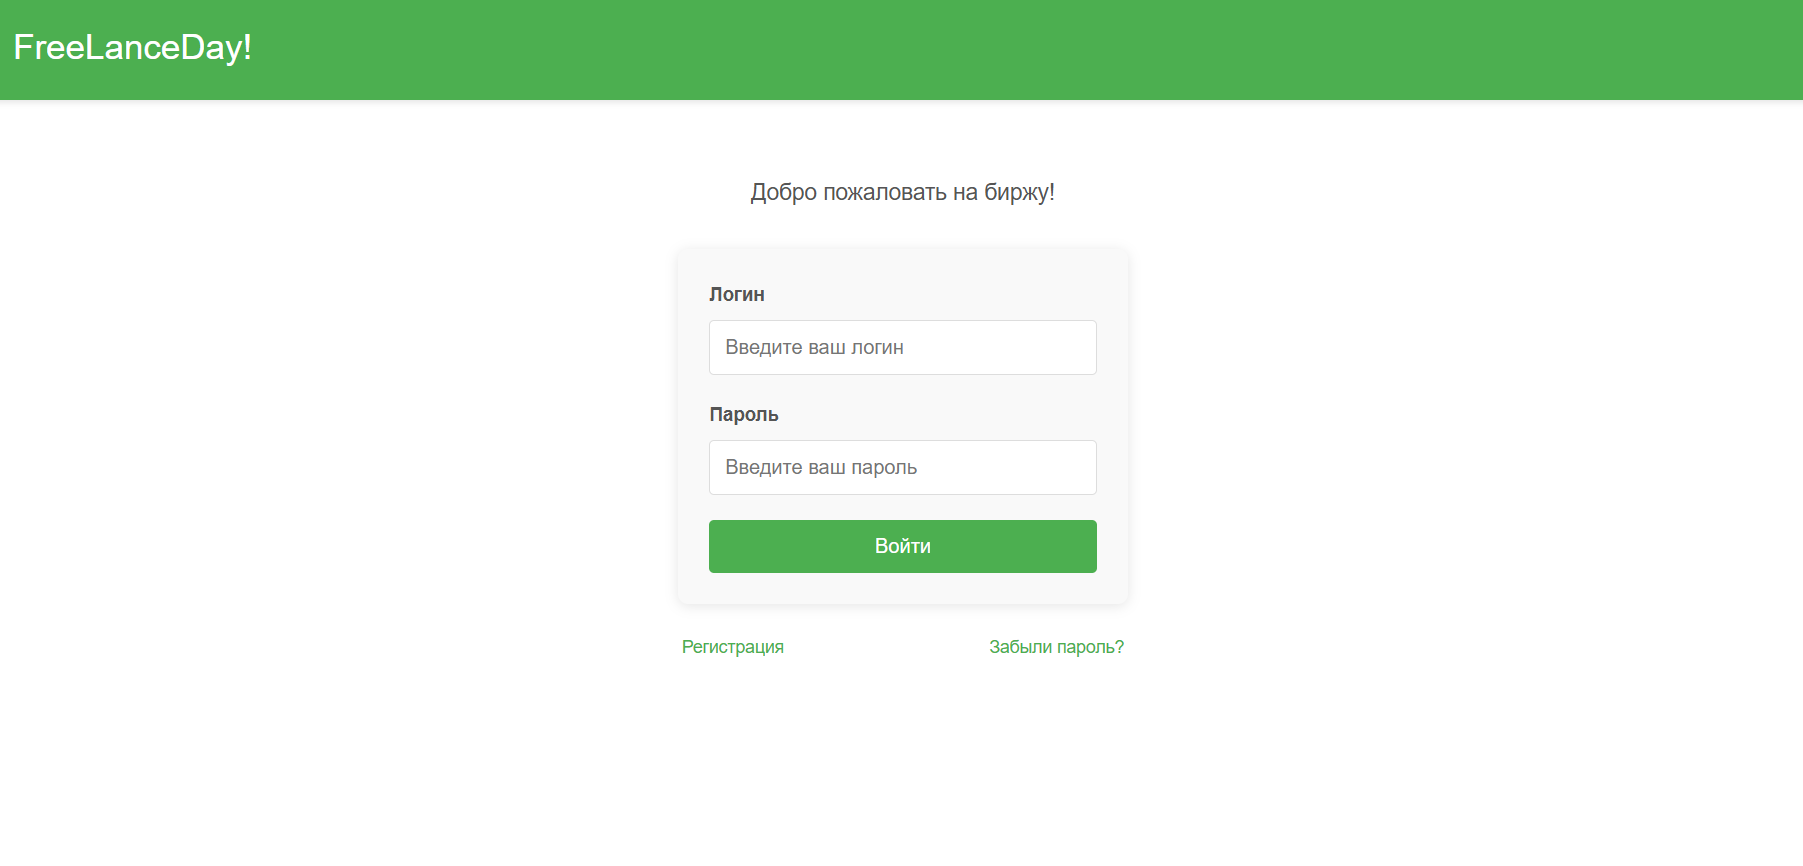
\includegraphics[width=1\linewidth]{t1.png}}
\caption{Страница авторизации сервиса}
\label{t1:image}
\end{figure}

На рисунках \ref{t2:image} и \ref{t3:image} представлена страница регистрации на сервисе с выбором типа регистрирующегося пользователя "<Заказчик"> и "<Исполнитель">.

\begin{figure}[ht]
\center{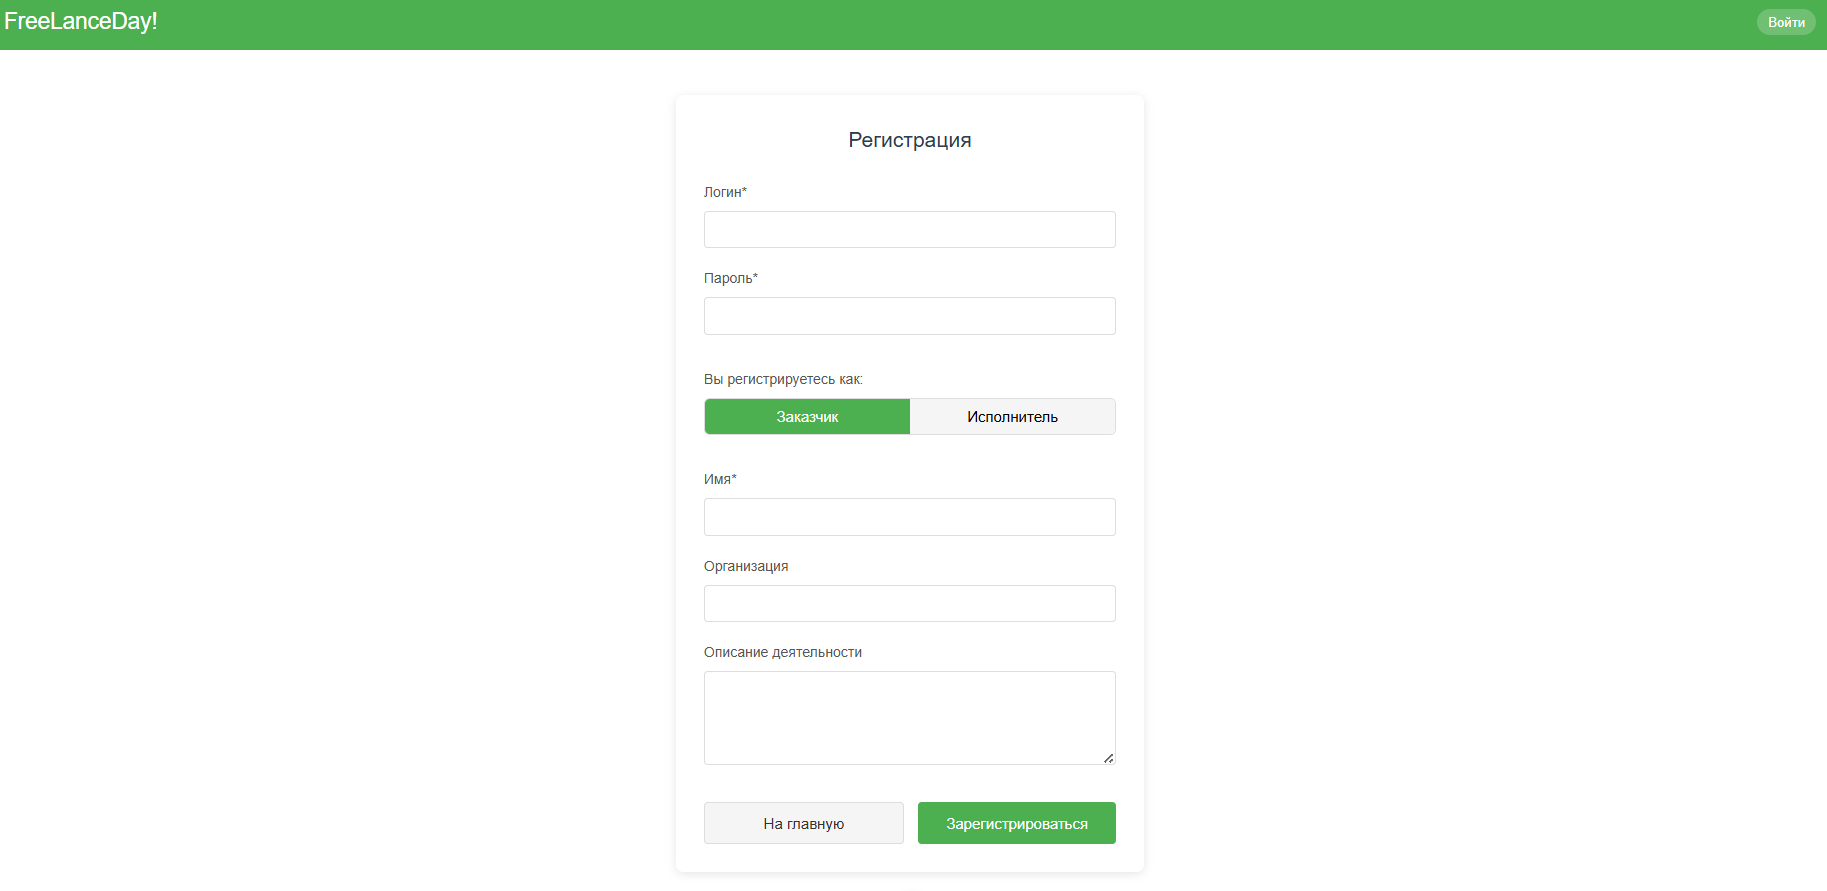
\includegraphics[width=1\linewidth]{t2.png}}
\caption{Страница регистрации для заказчика}
\label{t2:image}
\end{figure}
\clearpage

\begin{figure}[ht]
	\center{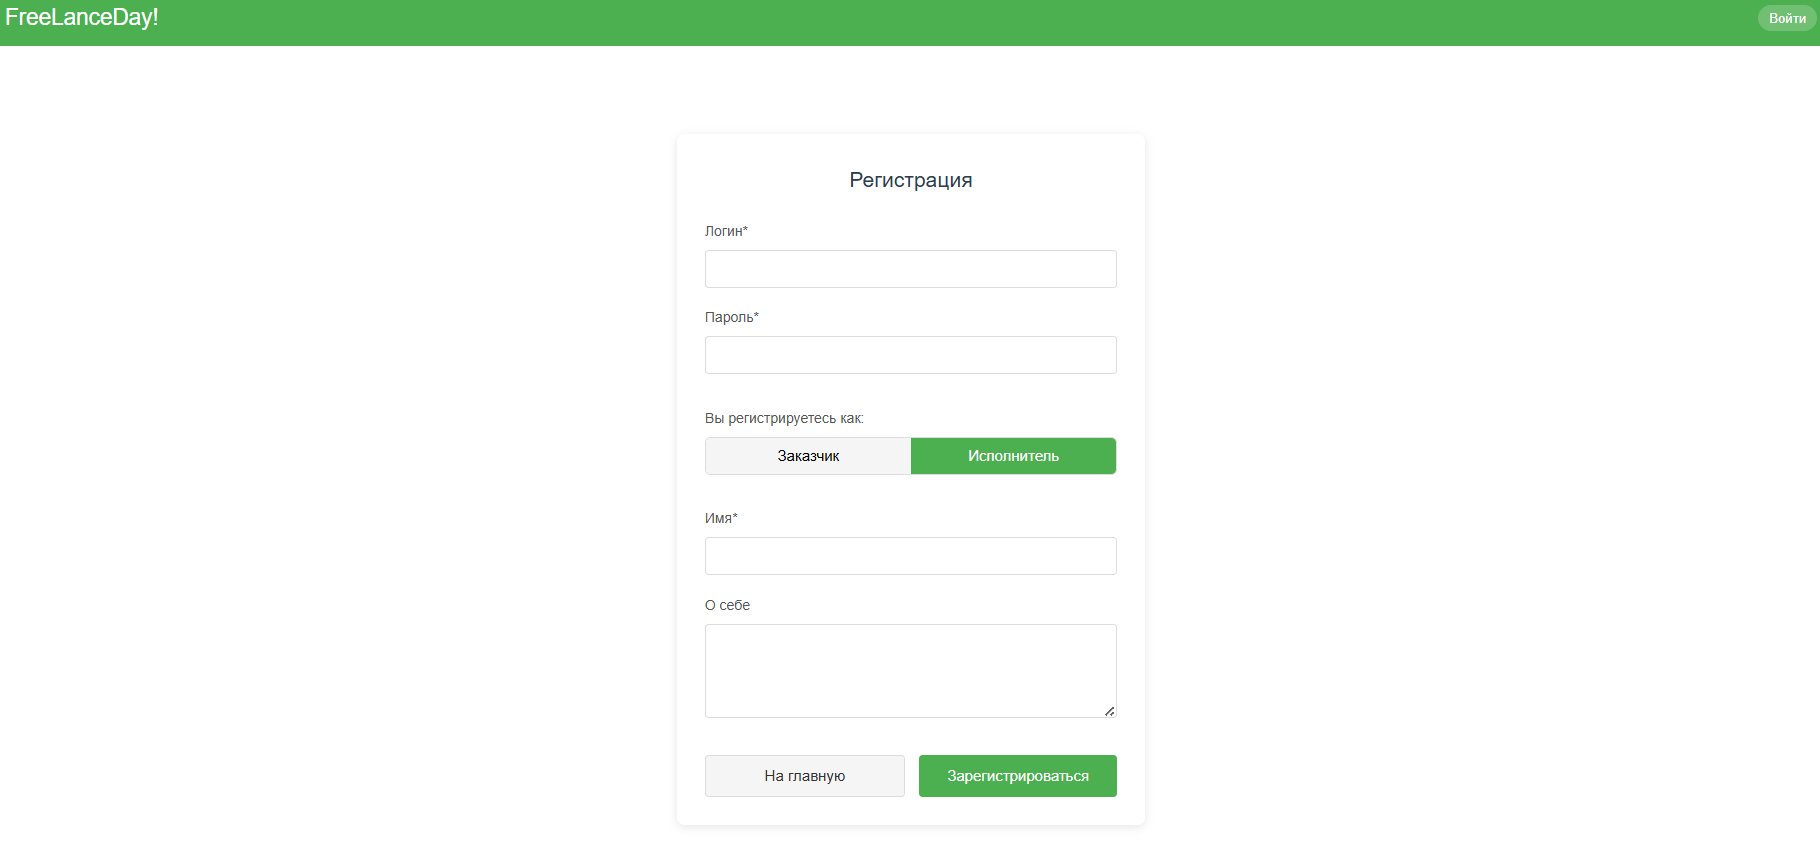
\includegraphics[width=1\linewidth]{t3.png}}
	\caption{Страница регистрации для исполнителя}
	\label{t3:image}
\end{figure}

На рисунках \ref{t4:image} и \ref{t5:image} представлена валидация полей на форме регистрации.

\begin{figure}[ht]
\center{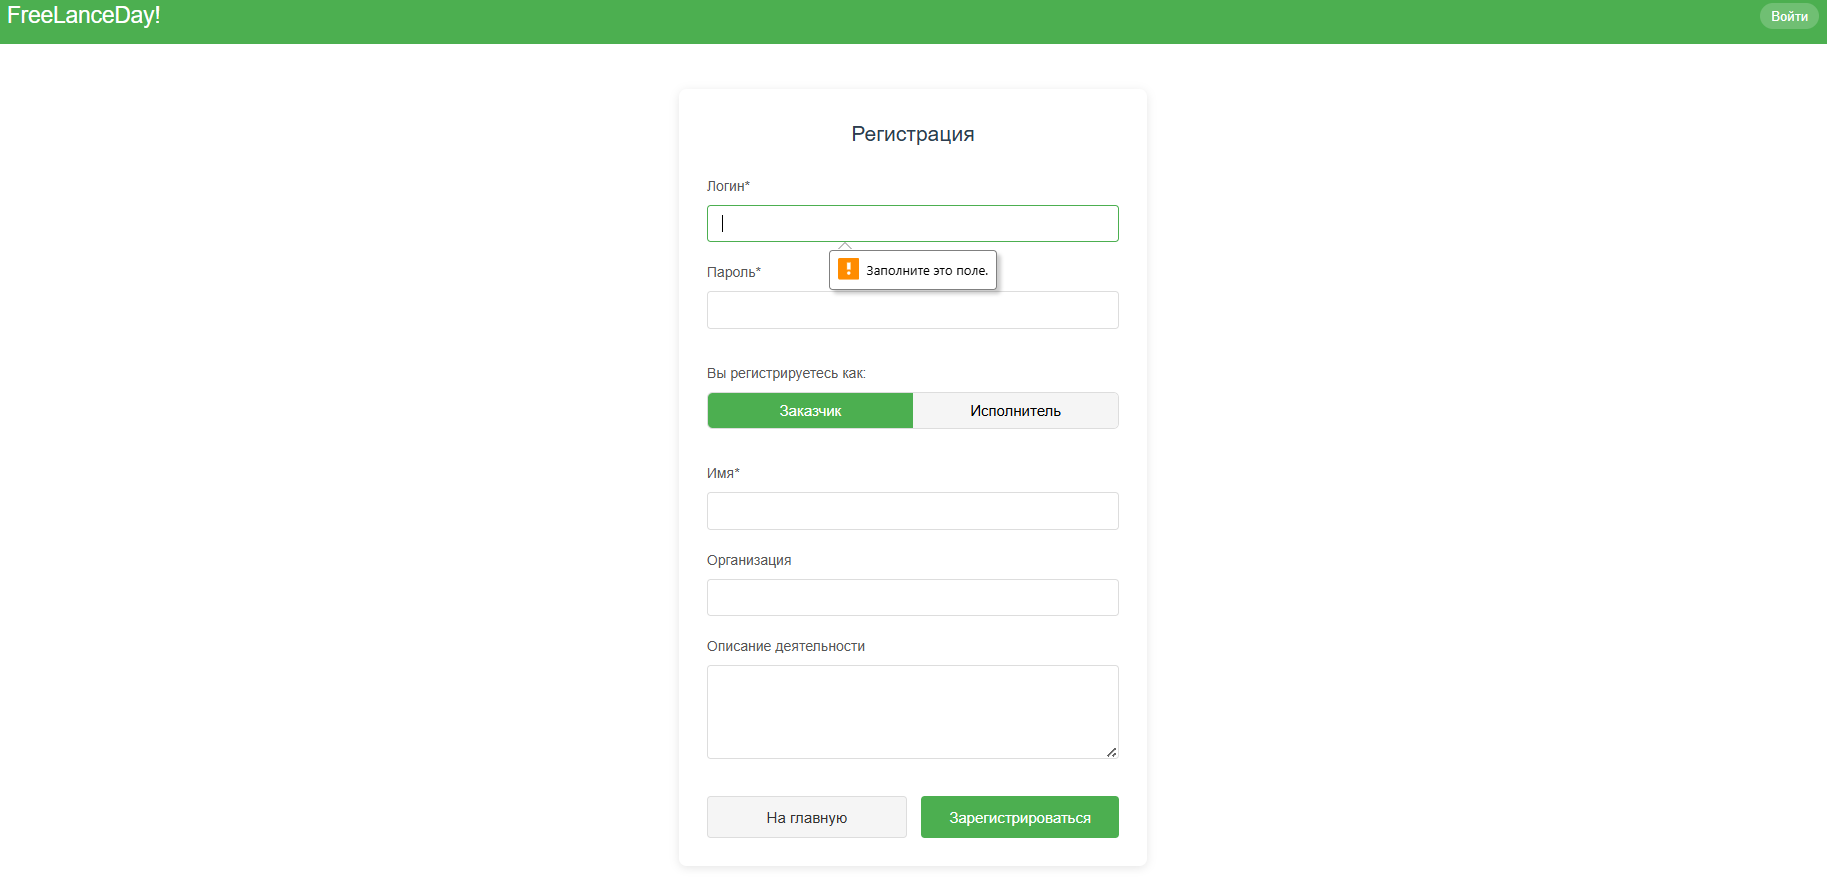
\includegraphics[width=1\linewidth]{t4.png}}
\caption{Валидация для поля "<Логин">}
\label{t4:image}
\end{figure}
\clearpage

\begin{figure}[ht]
	\center{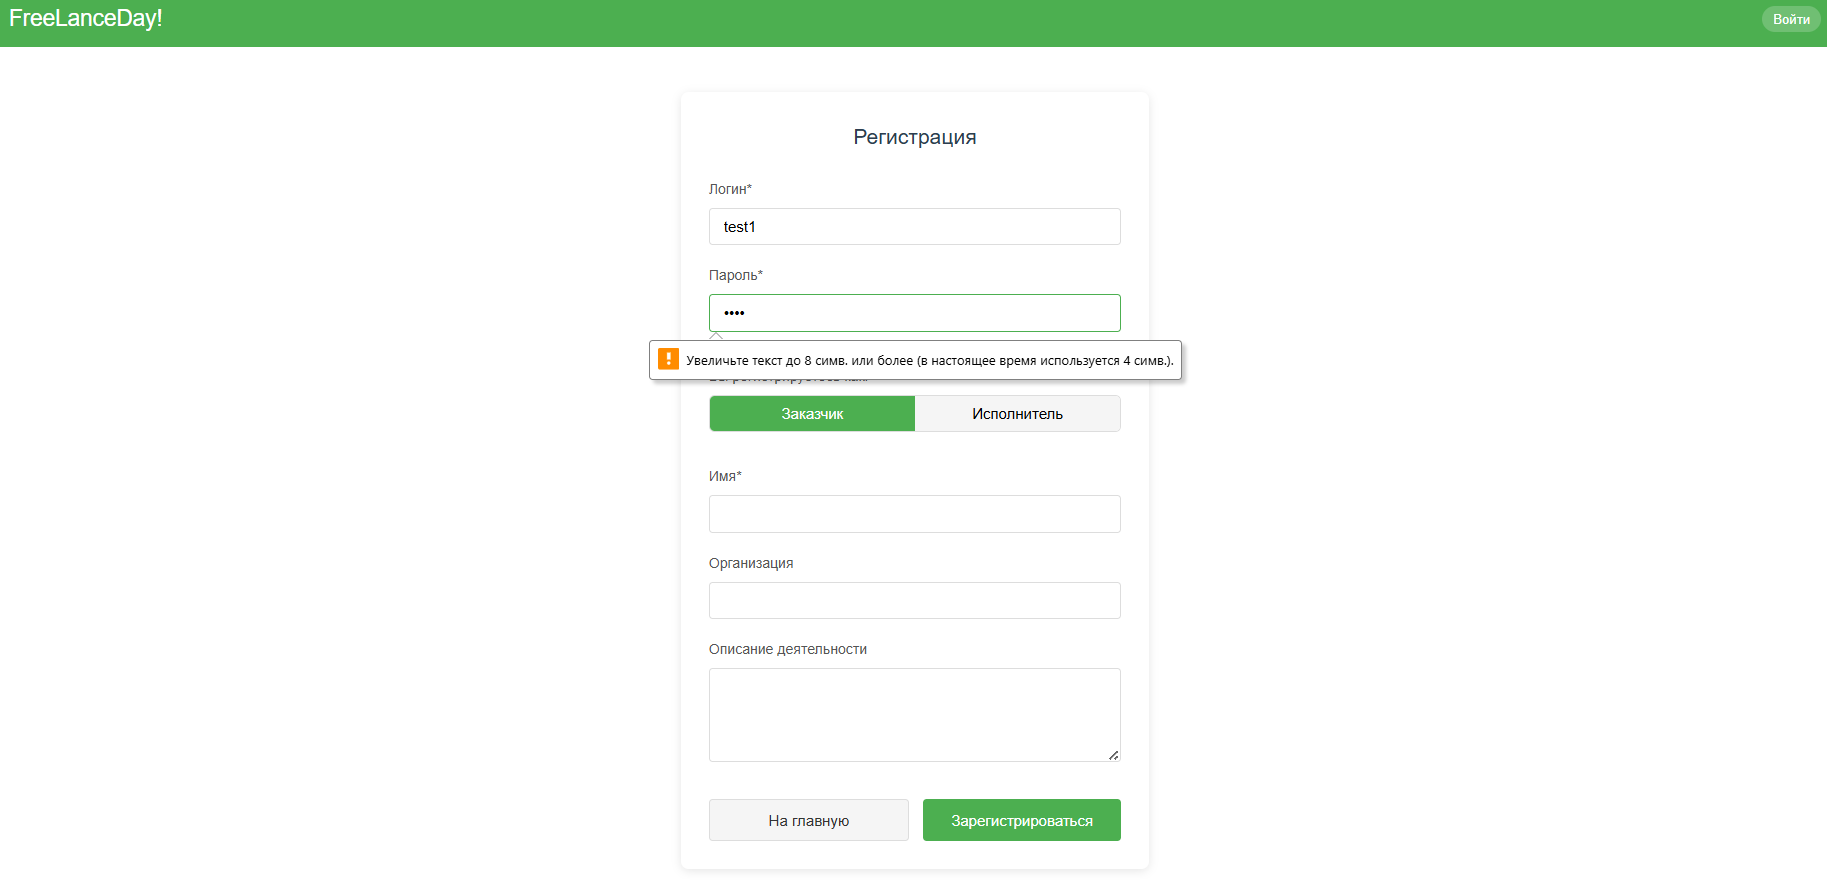
\includegraphics[width=1\linewidth]{t5.png}}
	\caption{Валидация для поля "<Пароль">}
	\label{t5:image}
\end{figure}

На рисунке \ref{t6:image} представлен пример успешной регистрации на сервисе.

\begin{figure}[ht]
	\center{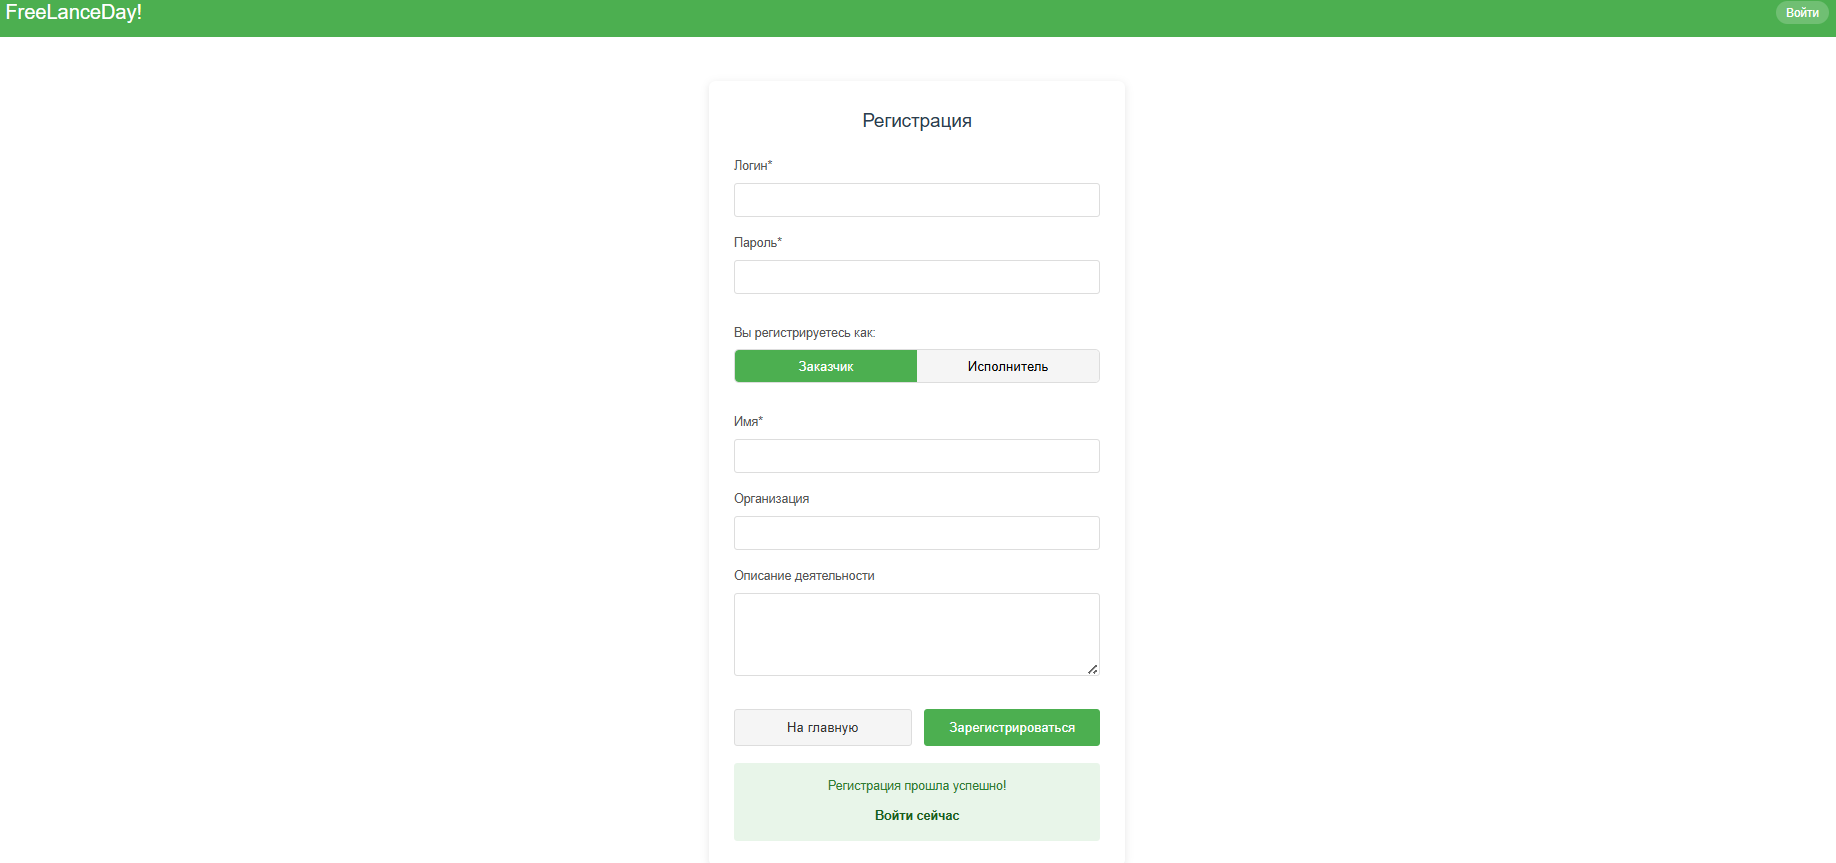
\includegraphics[width=1\linewidth]{t6.png}}
	\caption{Успешная регистрация на сервисе}
	\label{t6:image}
\end{figure}

На рисунках \ref{t7:image} и \ref{t8:image} представлен пример успешного входа в аккаунт пользователя с ролью "<Заказчик">.

\begin{figure}[ht]
	\center{
\includegraphics[width=1\linewidth]{t7.png}}
	\caption{Ввод авторизационных данных на странице авторизации}
	\label{t7:image}
\end{figure}

\begin{figure}[ht]
	\center{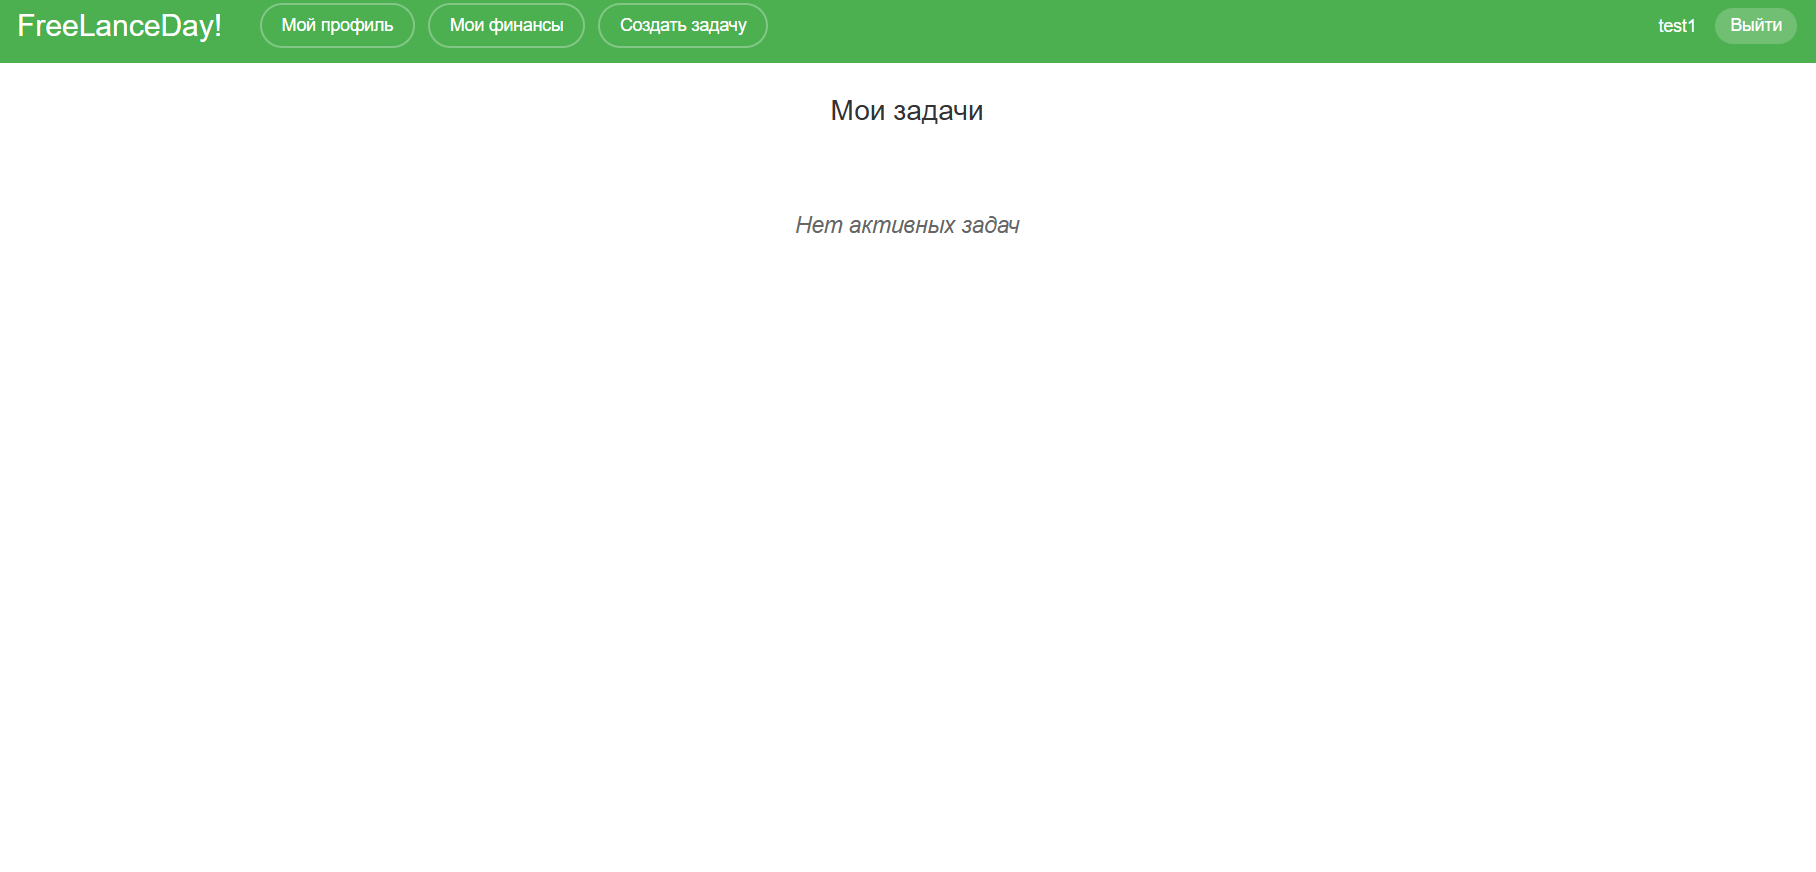
\includegraphics[width=1\linewidth]{t8.png}}
	\caption{Успешный вход на сервис}
	\label{t8:image}
\end{figure}
\clearpage

На рисунке \ref{t9:image} представлена личная страница пользователя.

\begin{figure}[ht]
	\center{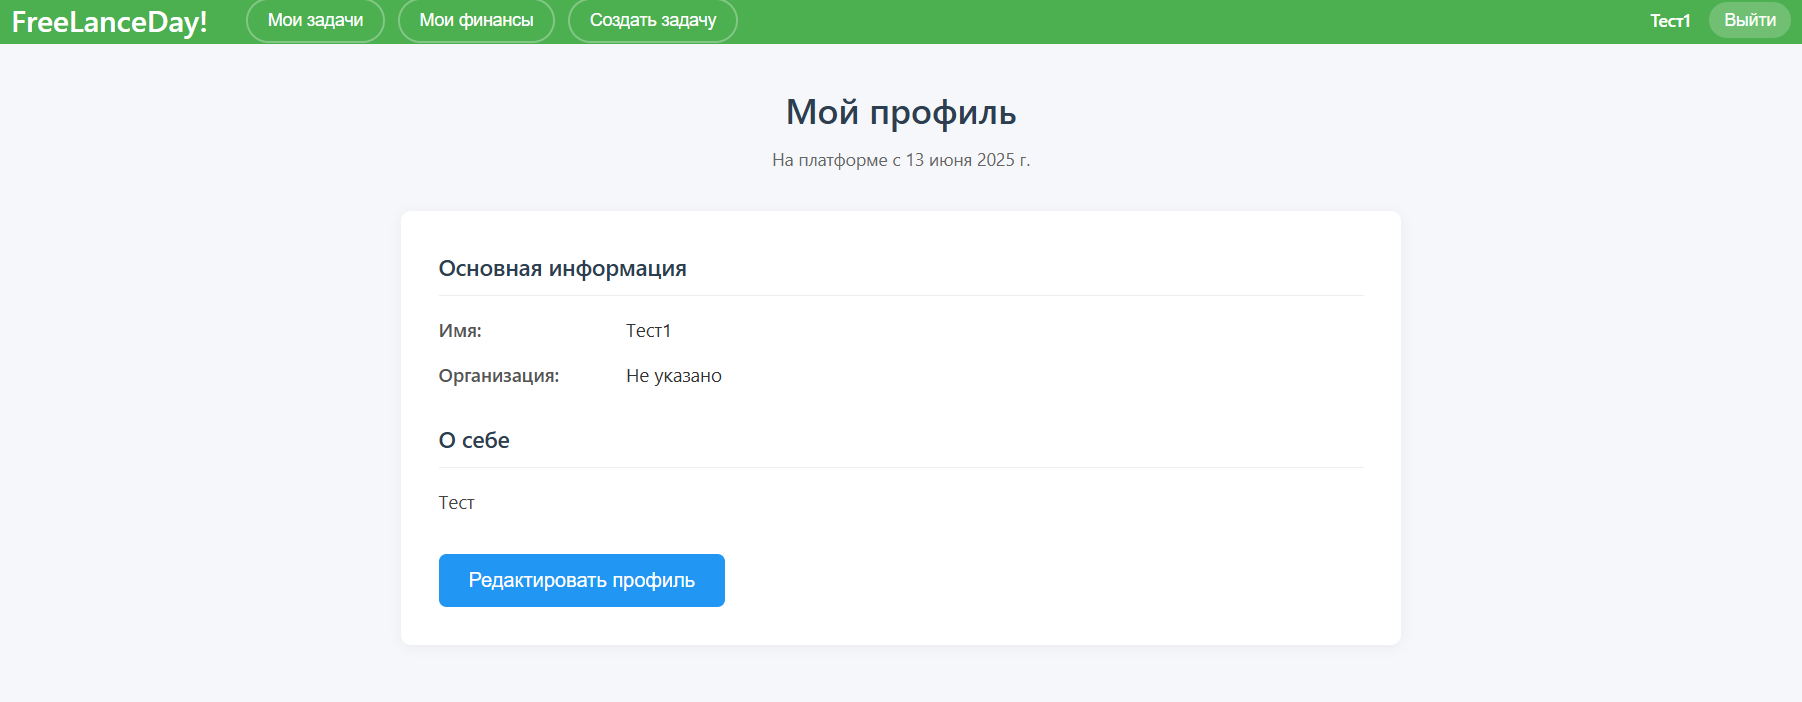
\includegraphics[width=1\linewidth]{t9.png}}
	\caption{Страница пользователя}
	\label{t9:image}
\end{figure}

На рисунке \ref{t10:image} представлена страница просмотра виртуального счёта пользователя.

\begin{figure}[ht]
	\center{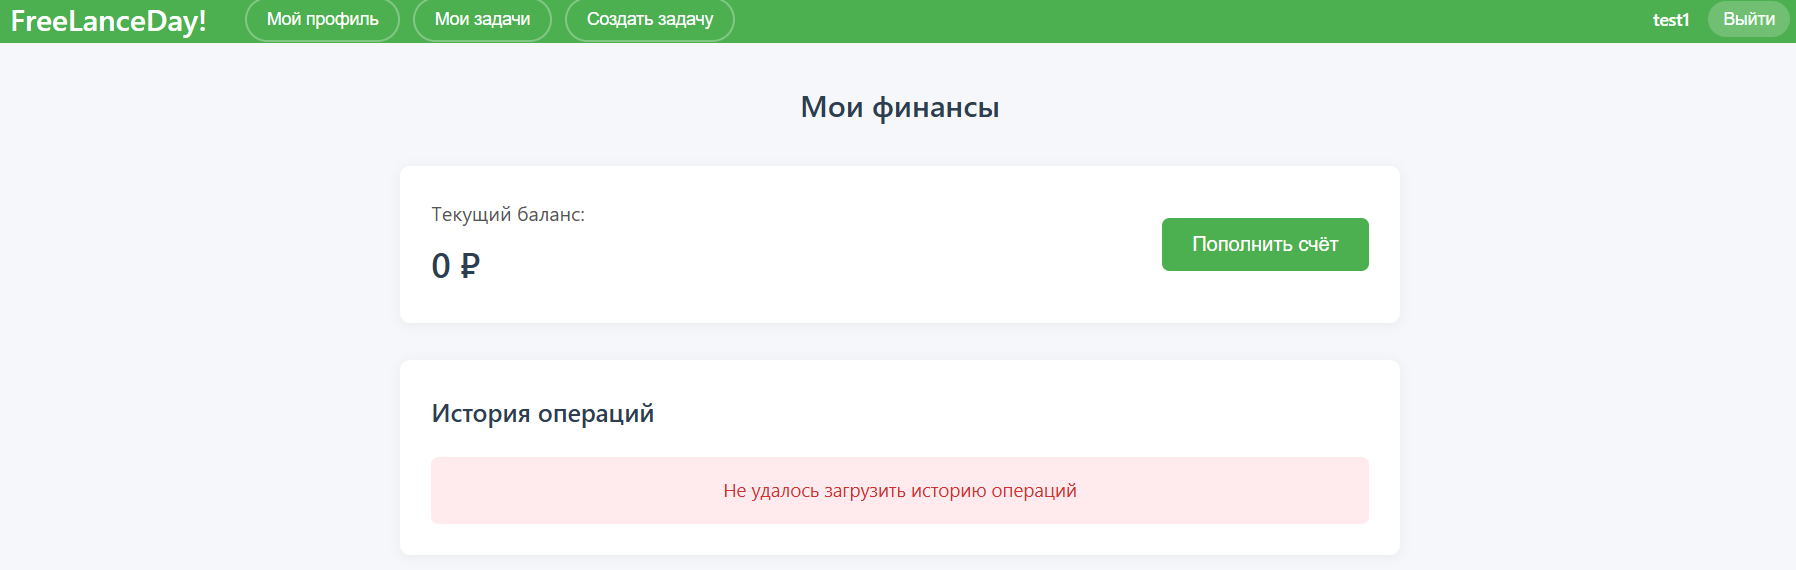
\includegraphics[width=1\linewidth]{t10.png}}
	\caption{Страница виртуального счёта пользователя}
	\label{t10:image}
\end{figure}

На рисунках \ref{t11:image}--\ref{t14:image} представлена страница пополнения виртуального счёта с различным заполнением полей.

\begin{figure}[ht]
	\center{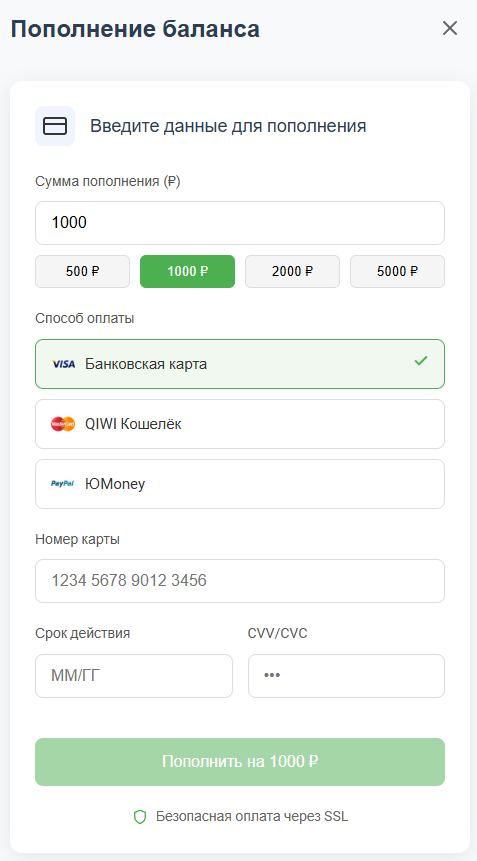
\includegraphics[width=0.7\linewidth]{t11.png}}
	\caption{Страница пополнения виртуального счёта}
	\label{t11:image}
\end{figure}

\begin{figure}[ht]
	\center{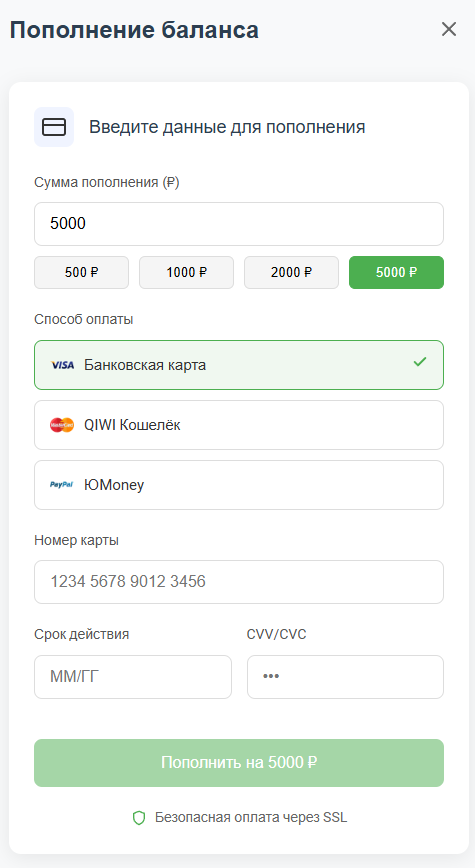
\includegraphics[width=0.7\linewidth]{t12.png}}
	\caption{Нажата кнопка "<5000Р">, поле с суммой пополнения заполнено соответствующим значением}
	\label{t12:image}
\end{figure}

\begin{figure}[ht]
	\center{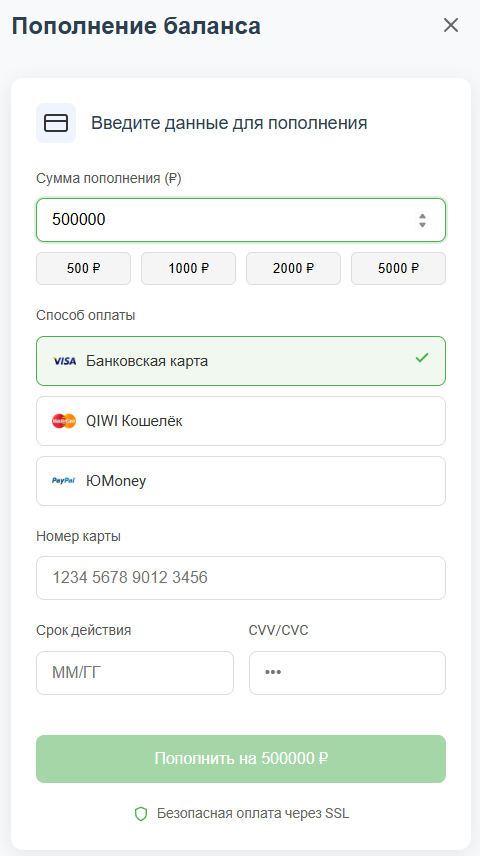
\includegraphics[width=0.7\linewidth]{t13.png}}
	\caption{Поле с суммой пополнения заполнено произвольным значением пользователя}
	\label{t13:image}
\end{figure}

\begin{figure}[ht]
	\center{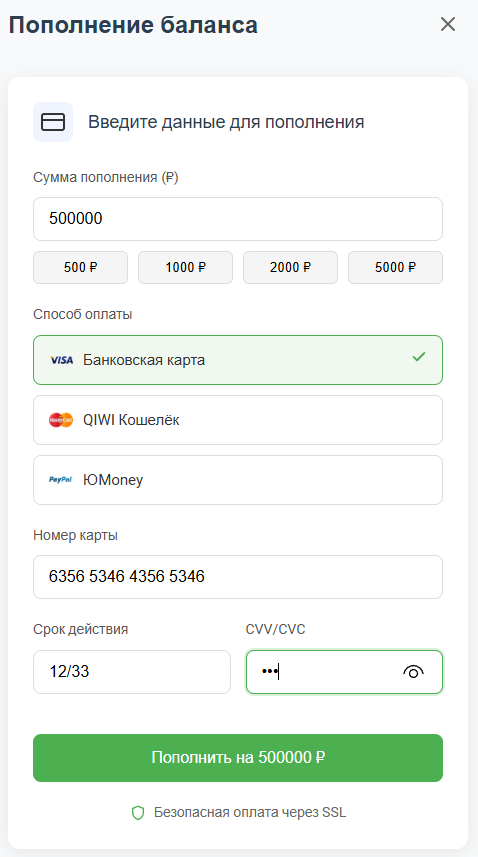
\includegraphics[width=0.7\linewidth]{t14.png}}
	\caption{Заполнены остальные обязательные поля, кнопка пополнения активна}
	\label{t14:image}
\end{figure}
\clearpage

На рисунках \ref{t15:image} и \ref{t16:image} представлено успешное пополнение виртуального счёта и последующий переход на страницу просмотра информации о счёте.

\begin{figure}[ht]
	\center{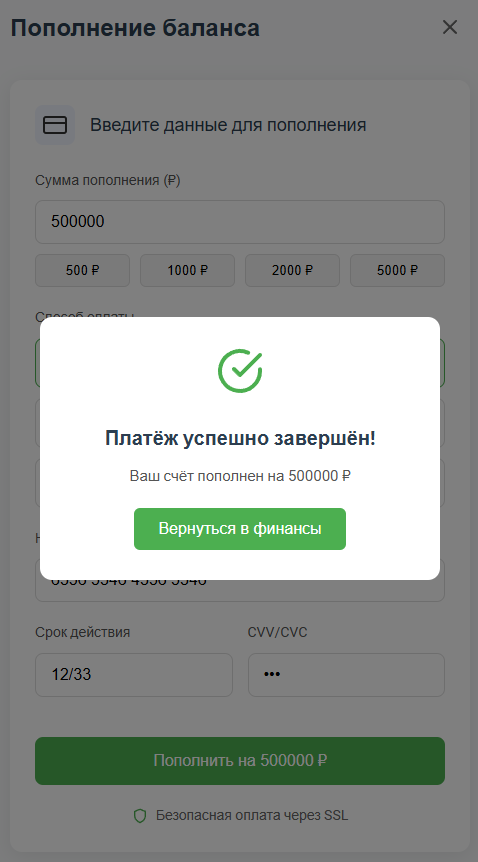
\includegraphics[width=0.7\linewidth]{t15.png}}
	\caption{Сообщение об успешном пополнении виртуального счёта}
	\label{t15:image}
\end{figure}

\begin{figure}[ht]
	\center{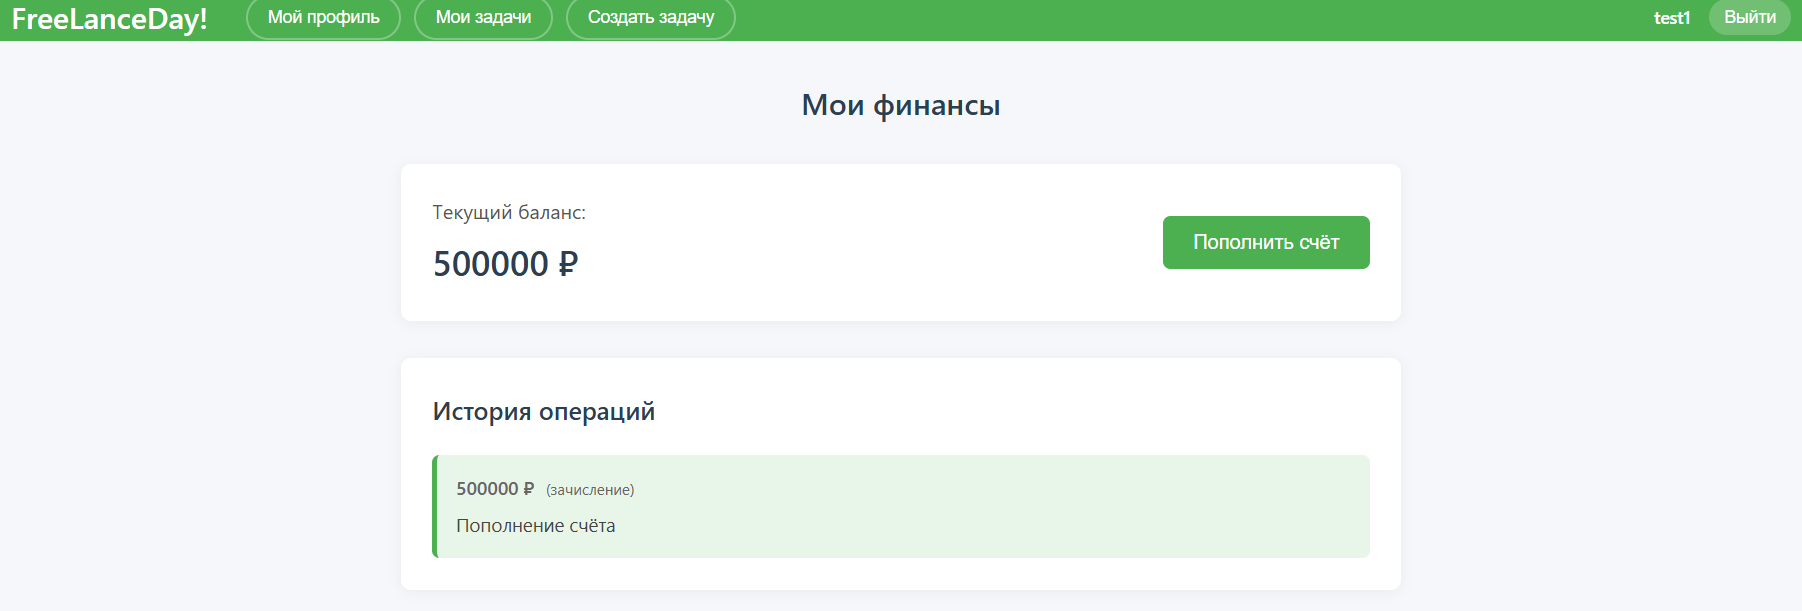
\includegraphics[width=1\linewidth]{t16.png}}
	\caption{Страница просмотра виртуального счёта, баланс соответствует сумме пополнения}
	\label{t16:image}
\end{figure}

На рисунках \ref{t17:image}, \ref{t18:image} и \ref{t19:image} представлена форма создания задачи с незаполненными полями, невалидным и валидным заполнением.

\begin{figure}[ht]
	\center{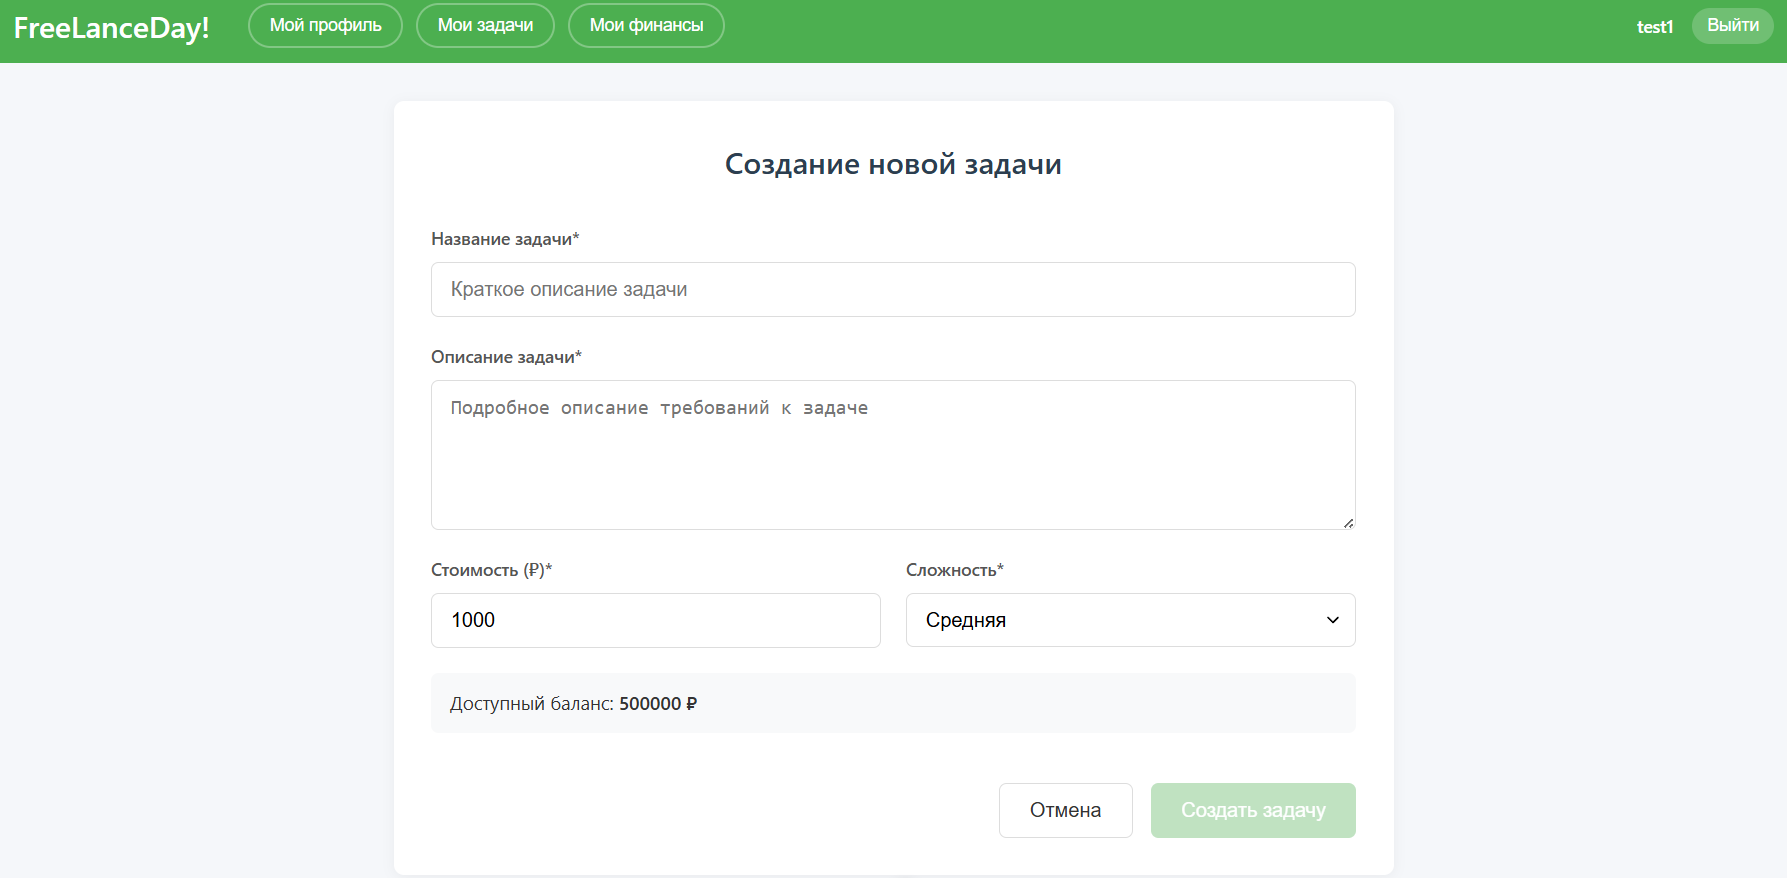
\includegraphics[width=1\linewidth]{t17.png}}
	\caption{Форма создания задачи}
	\label{t17:image}
\end{figure}

\begin{figure}[ht]
	\center{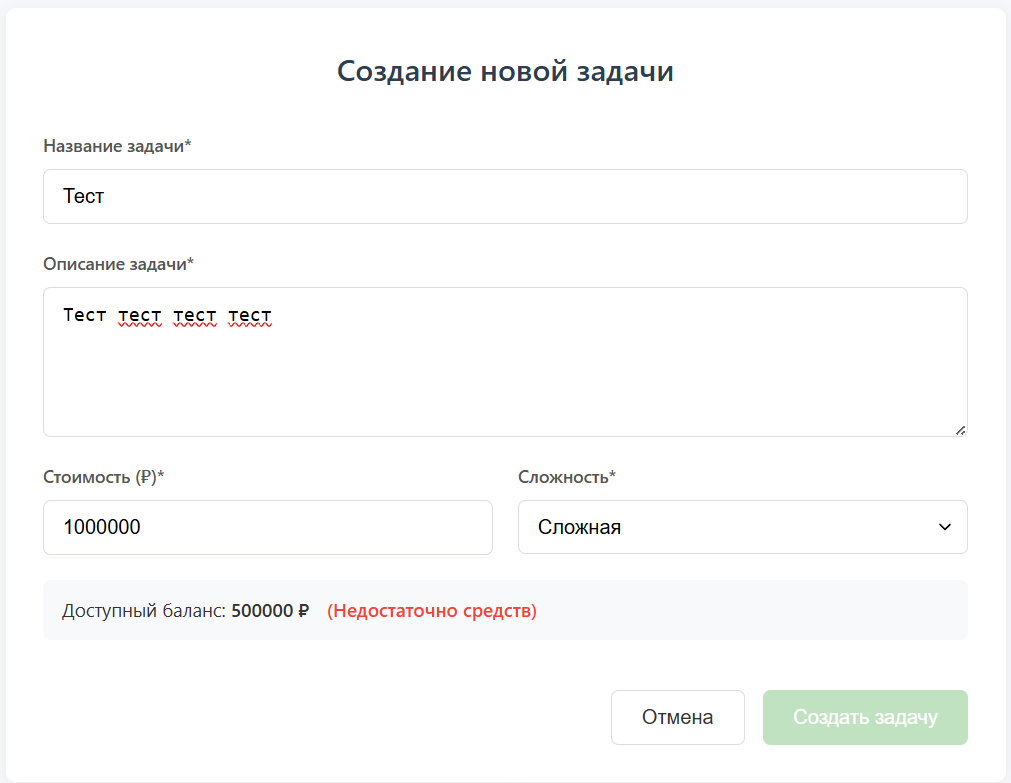
\includegraphics[width=1\linewidth]{t18.png}}
	\caption{Невалидное заполнение формы}
	\label{t18:image}
\end{figure}
\clearpage

\begin{figure}[ht]
	\center{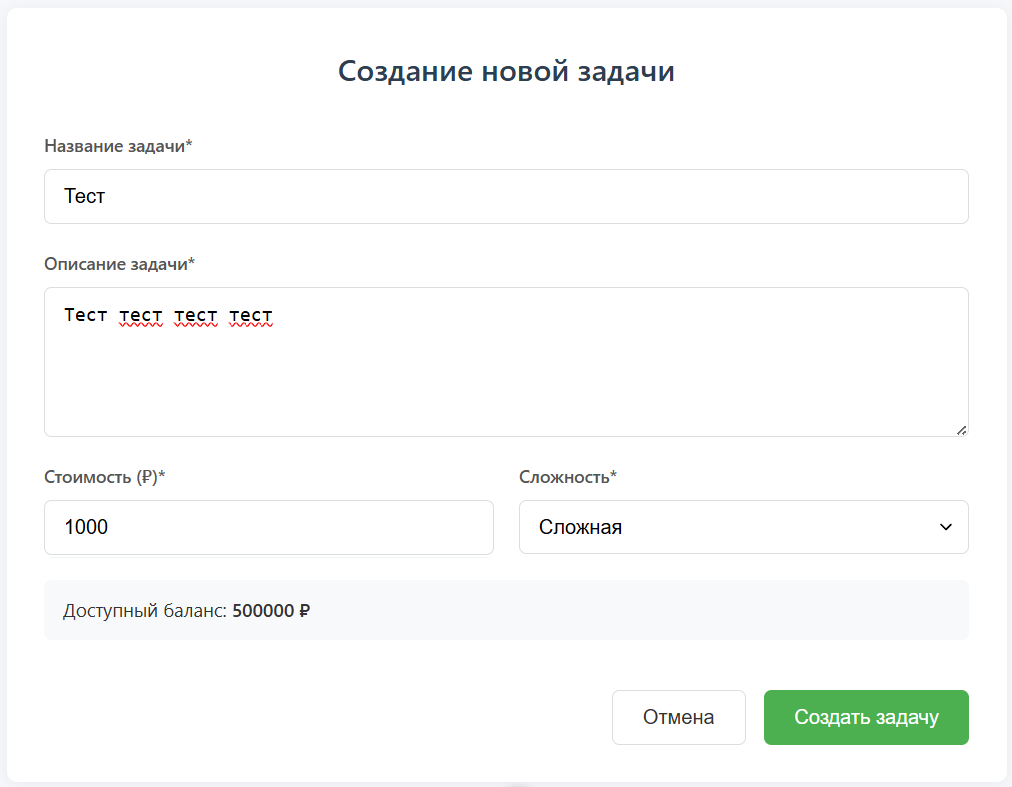
\includegraphics[width=1\linewidth]{t19.png}}
	\caption{Валидное заполнение формы}
	\label{t19:image}
\end{figure}


На рисунках \ref{t20:image} и \ref{t21:image} представлены страница просмотра задач пользователя и страница просмотра конкретной задачи.

\begin{figure}[ht]
	\center{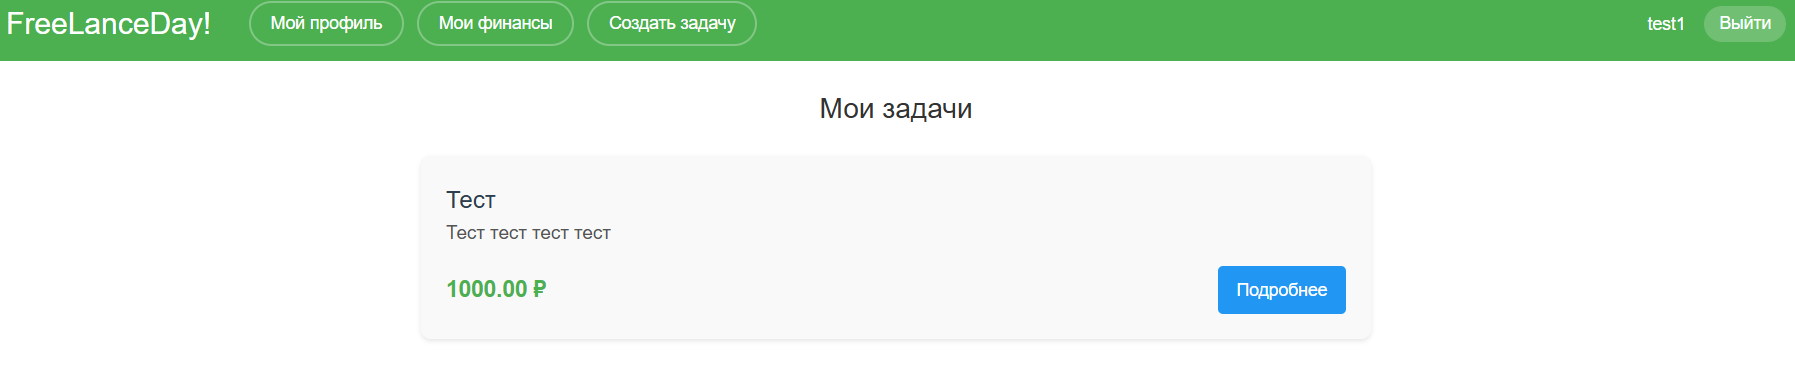
\includegraphics[width=1\linewidth]{t20.png}}
	\caption{Страница просмотра списка задач пользователя}
	\label{t20:image}
\end{figure}
\clearpage

\begin{figure}[ht]
	\center{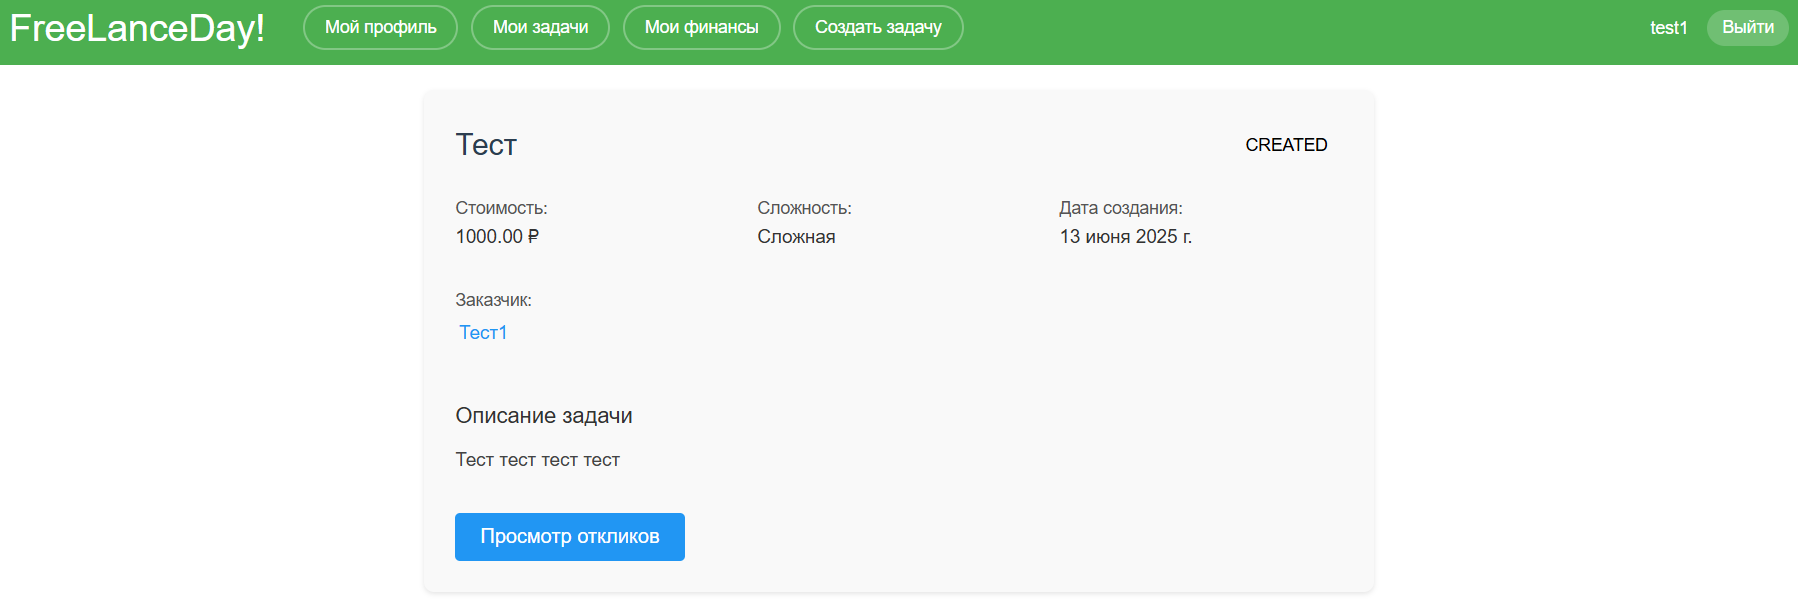
\includegraphics[width=1\linewidth]{t21.png}}
	\caption{Страница просмотра информации о созданной задаче с профиля создавшего пользователя}
	\label{t21:image}
\end{figure}

На рисунках \ref{t22:image} и \ref{t23:image} представлены страница просмотра профиля заказчика задачи и страница просмотра откликов на задачу.

\begin{figure}[ht]
	\center{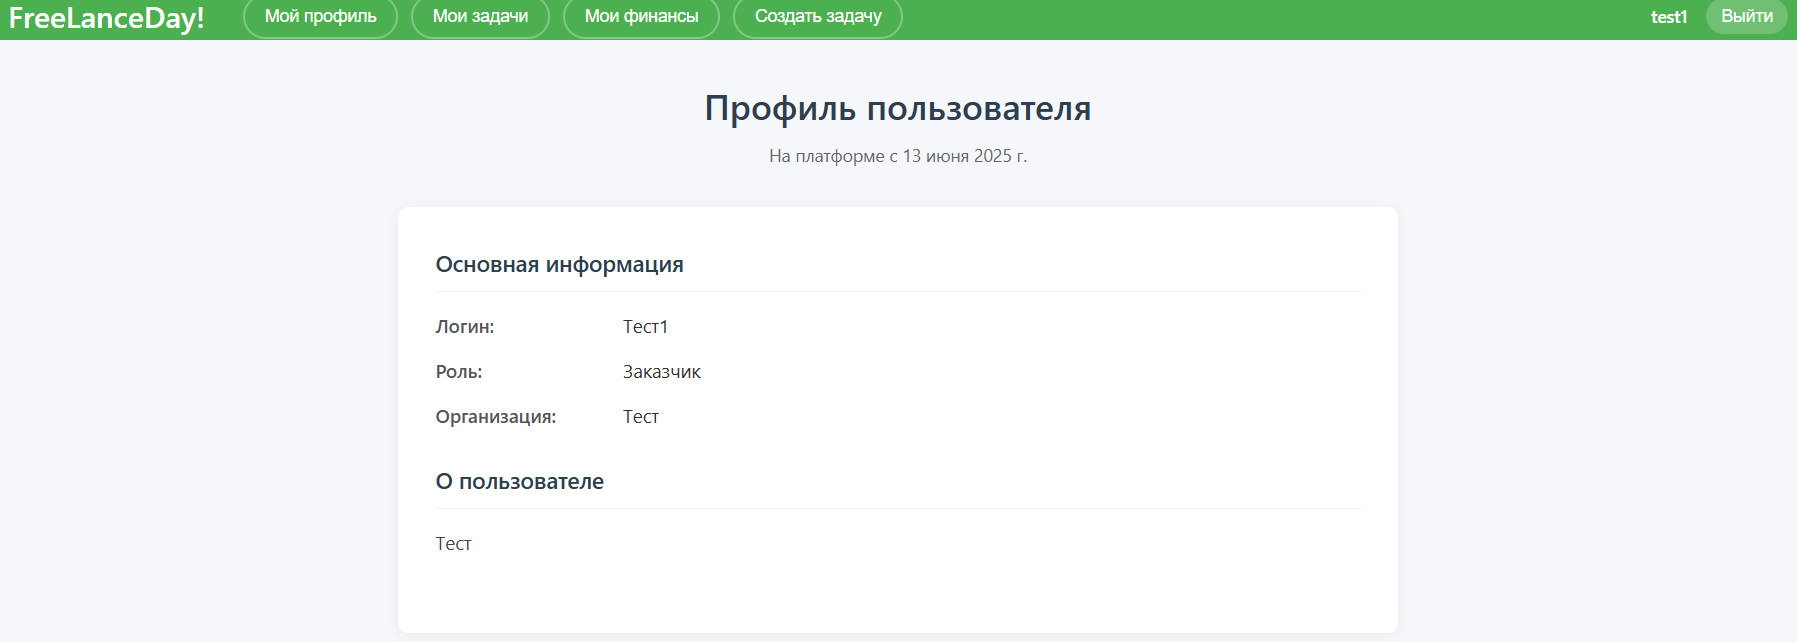
\includegraphics[width=1\linewidth]{t22.png}}
	\caption{Страница просмотра профиля заказчика задачи}
	\label{t22:image}
\end{figure}

\begin{figure}[ht]
	\center{
\includegraphics[width=1\linewidth]{t23.png}}
	\caption{Страница просмотра откликов на задачу}
	\label{t23:image}
\end{figure}
\clearpage

На рисунках \ref{t24:image} и \ref{t25:image} представлен вход на сервис с аккаунта исполнителя.

\begin{figure}[ht]
	\center{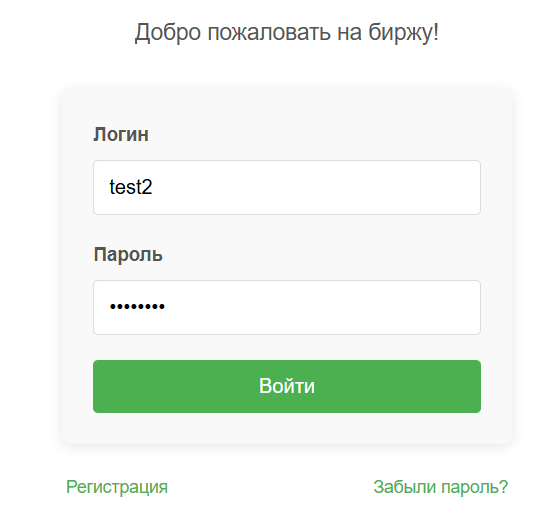
\includegraphics[width=0.5\linewidth]{t24.png}}
	\caption{Страница авторизации с введёнными данными исполнителя}
	\label{t24:image}
\end{figure}

\begin{figure}[ht]
	\center{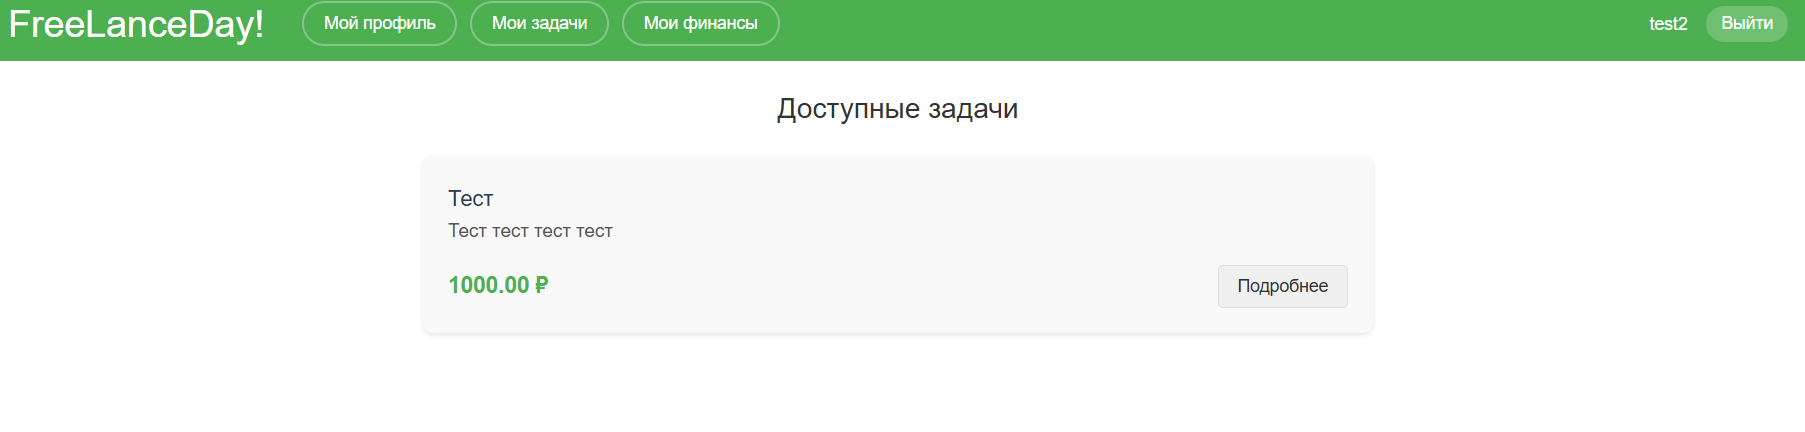
\includegraphics[width=1\linewidth]{t25.png}}
	\caption{Исполнителем осуществлён вход, отображается страница поиска задач}
	\label{t25:image}
\end{figure}

На рисунке \ref{t26:image} представлена страниц просмотра своего профиля исполнителем.
\clearpage

\begin{figure}[ht]
	\center{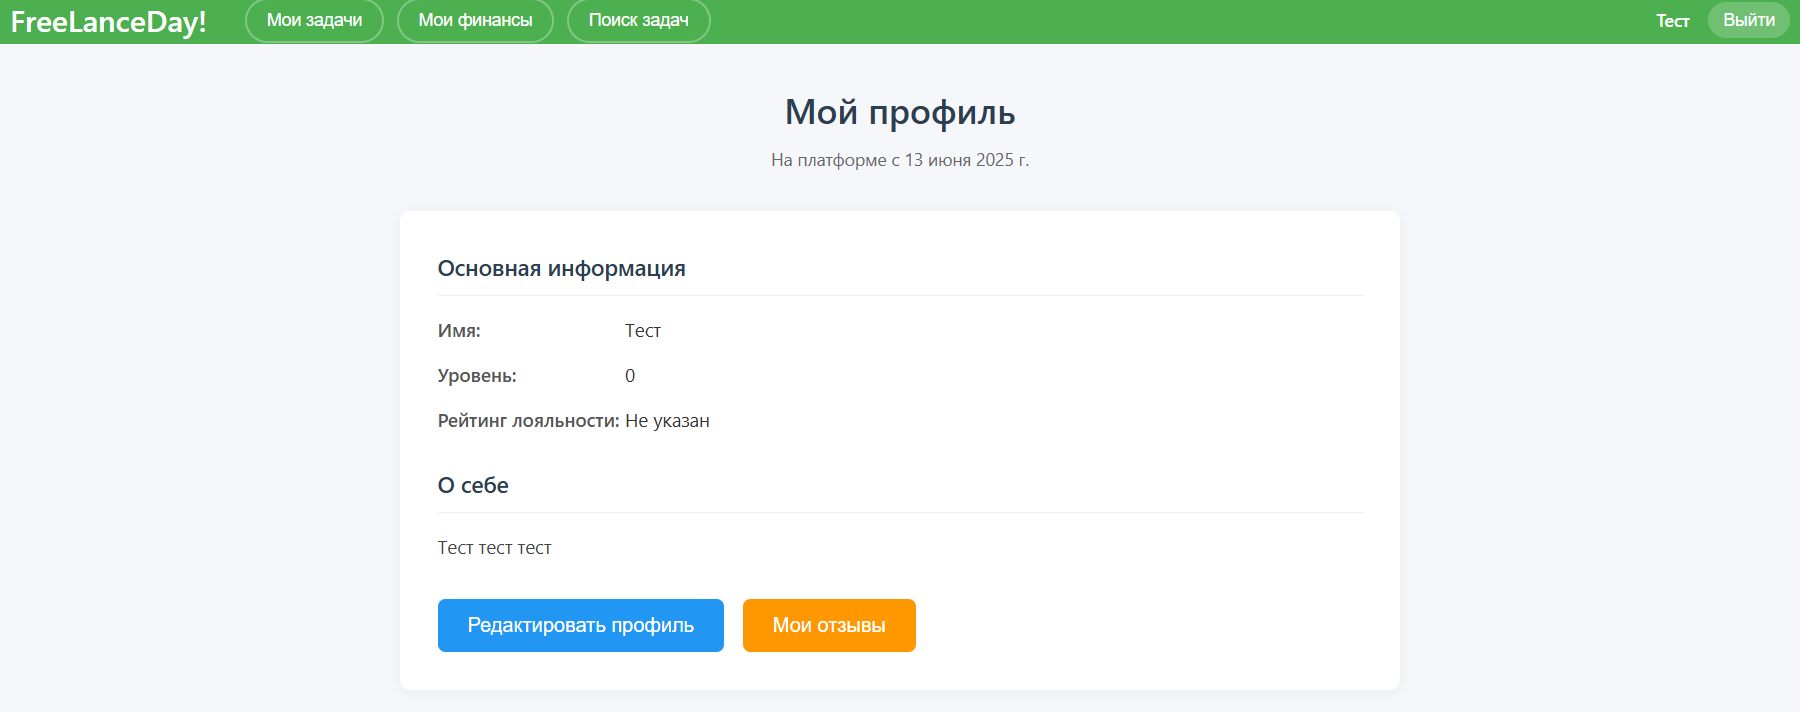
\includegraphics[width=1\linewidth]{t26.png}}
	\caption{Страница просмотра своего профиля исполнителем}
	\label{t26:image}
\end{figure}

На рисунках \ref{t27:image}, \ref{t28:image} и \ref{t29:image} представлена страница просмотра задачи исполнителем и отклик на неё.

\begin{figure}[ht]
	\center{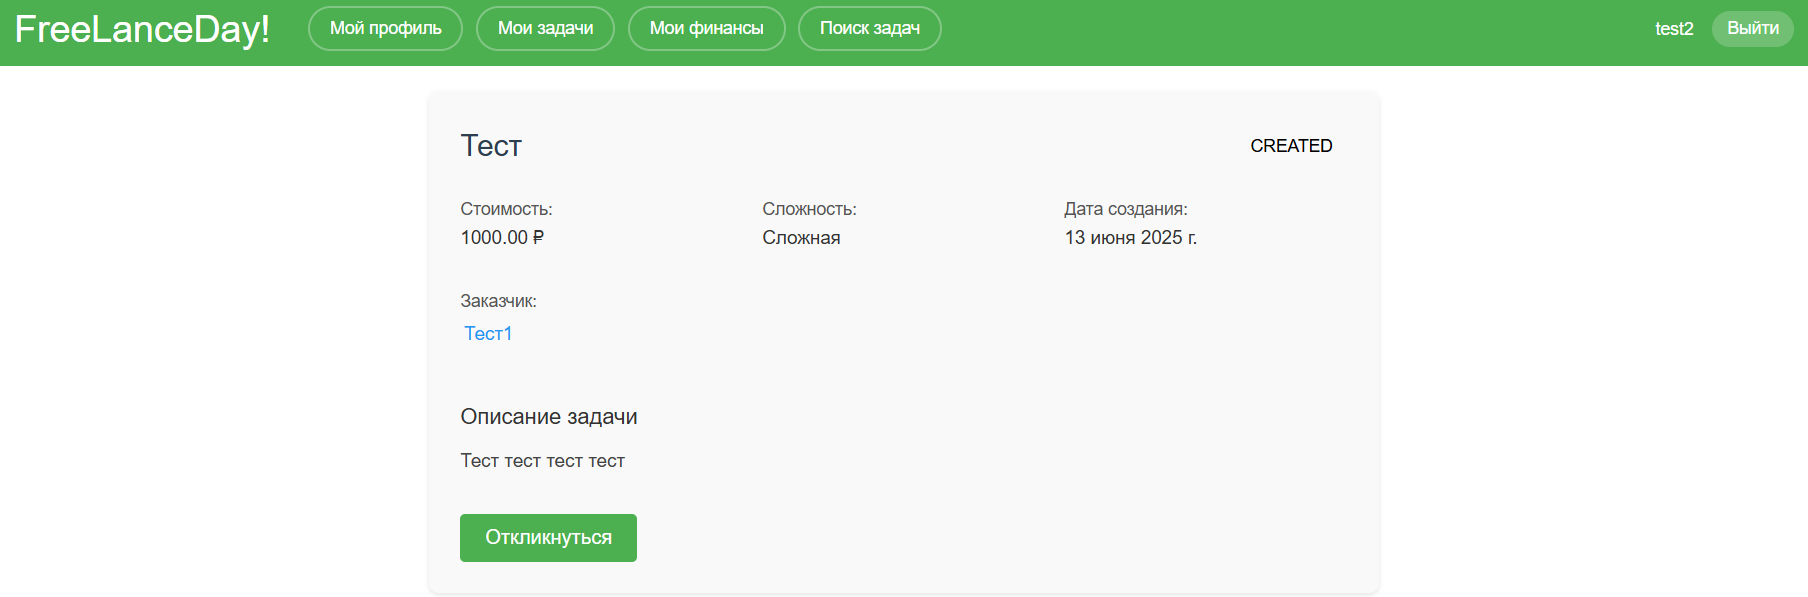
\includegraphics[width=1\linewidth]{t27.png}}
	\caption{Просмотр задачи исполнителем}
	\label{t27:image}
\end{figure}

\begin{figure}[ht]
	\center{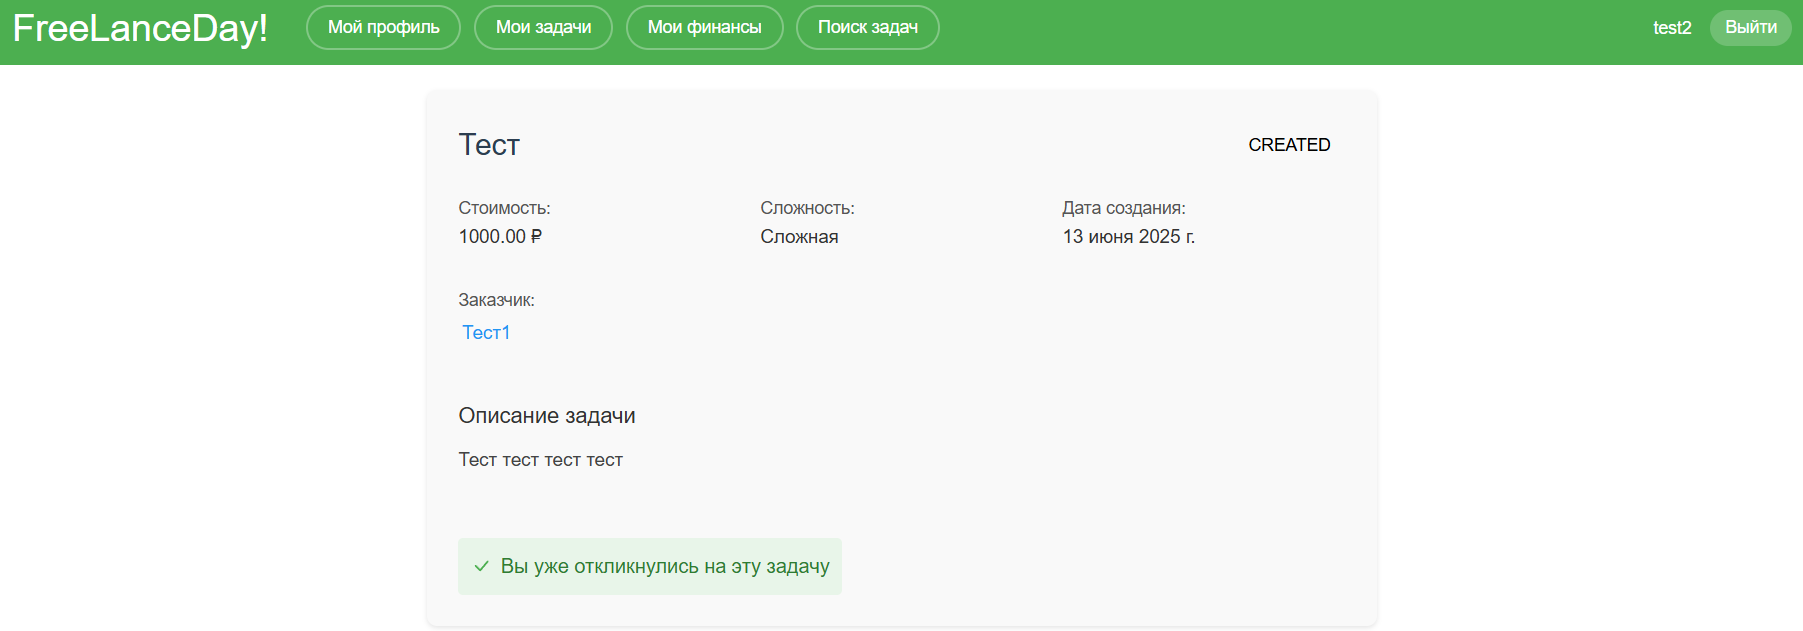
\includegraphics[width=1\linewidth]{t28.png}}
	\caption{Отклик на задачу}
	\label{t28:image}
\end{figure}

\begin{figure}[ht]
	\center{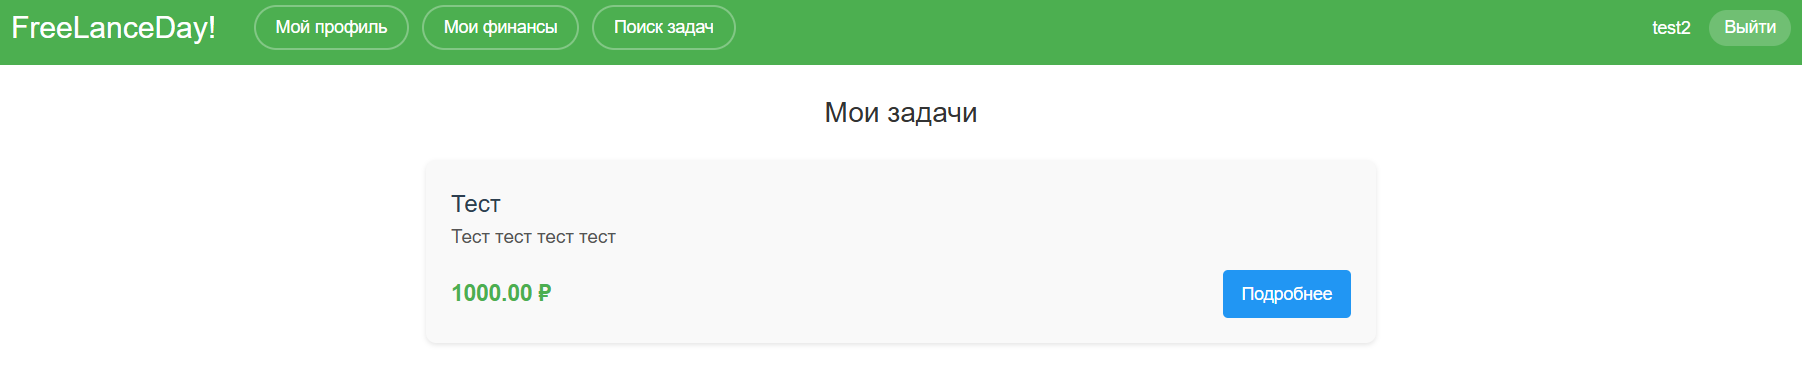
\includegraphics[width=1\linewidth]{t29.png}}
	\caption{Задача отображается в разделе "<Мои задачи"> откликнувшегося исполнителя}
	\label{t29:image}
\end{figure}

На рисунках \ref{t30:image}--\ref{t34:image} представлено назначение откликнувшегося исполнителя на задачу.

\begin{figure}[ht]
	\center{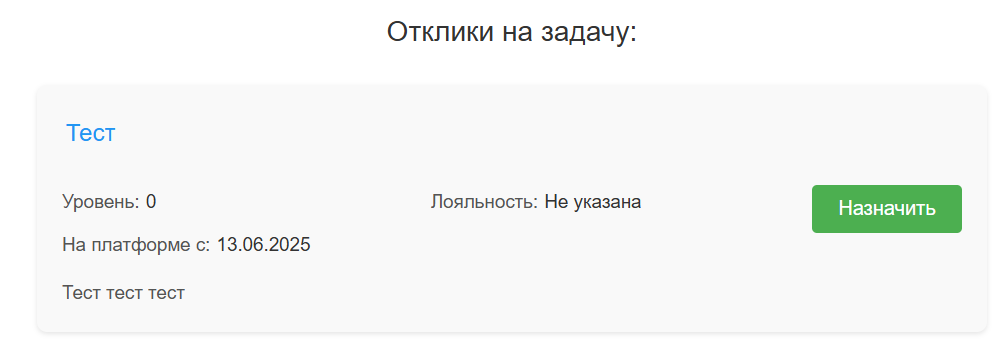
\includegraphics[width=1\linewidth]{t30.png}}
	\caption{Просмотр откликнувшихся исполнителей на задачу}
	\label{t30:image}
\end{figure}

\begin{figure}[ht]
	\center{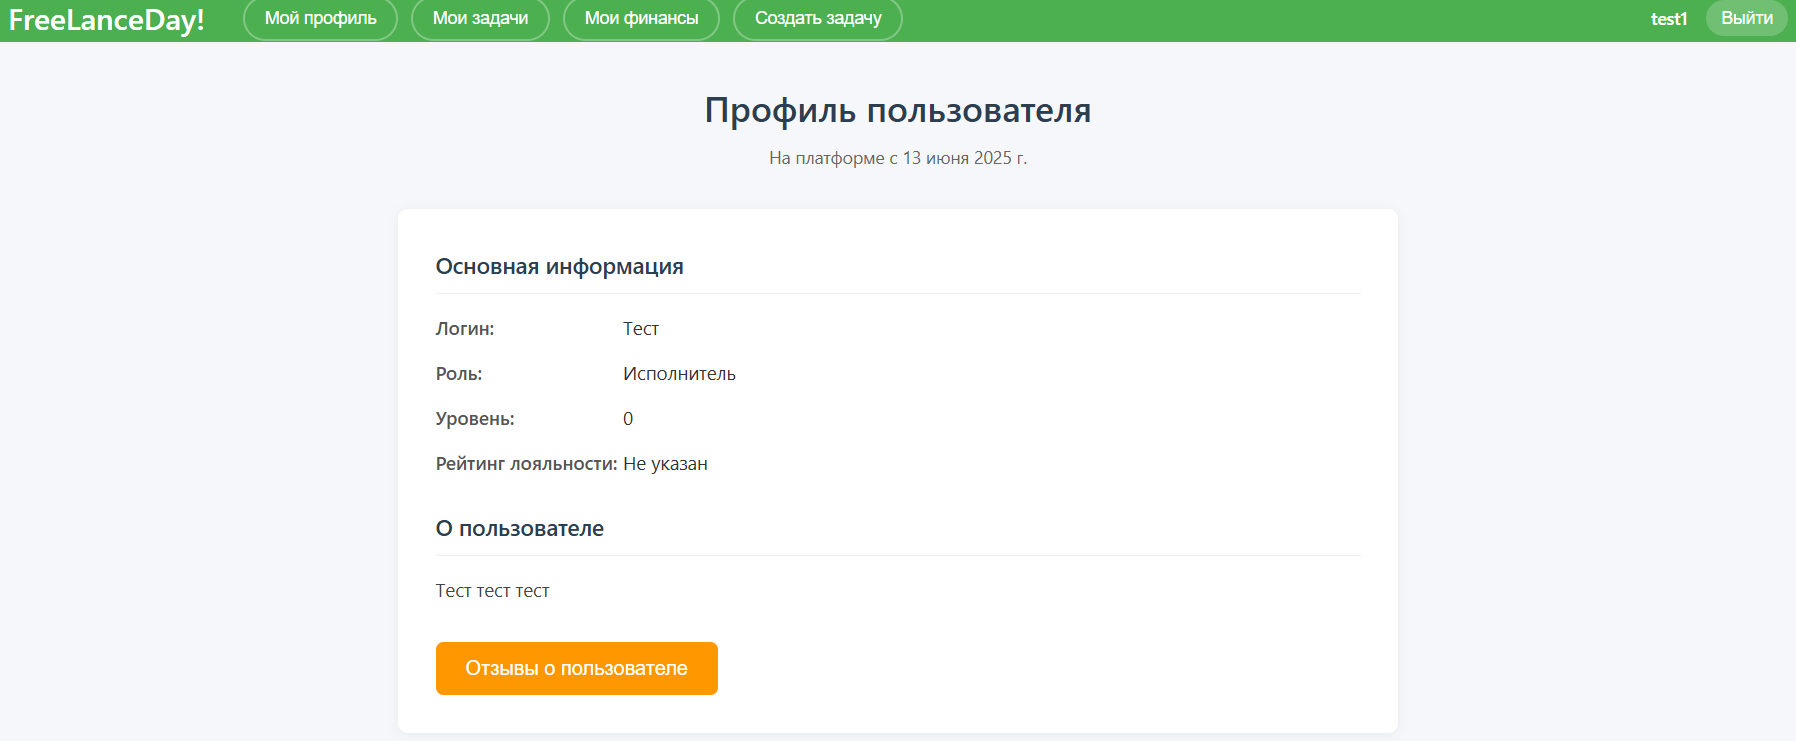
\includegraphics[width=1\linewidth]{t31.png}}
	\caption{Просмотр профиля откликнувшегося исполнителя}
	\label{t31:image}
\end{figure}

\begin{figure}[ht]
	\center{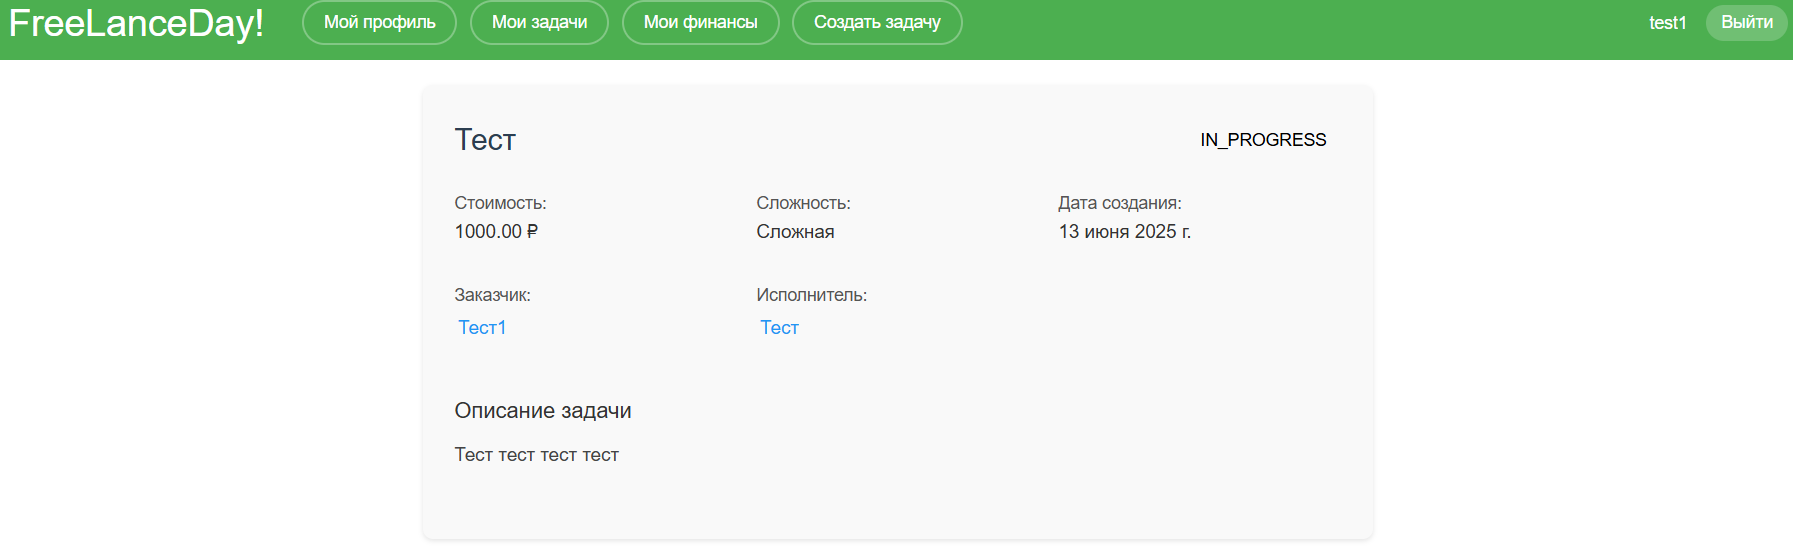
\includegraphics[width=1\linewidth]{t32.png}}
	\caption{Исполнитель успешно назначен на задачу}
	\label{t32:image}
\end{figure}

\begin{figure}[ht]
	\center{
\includegraphics[width=0.5\linewidth]{t34.png}}
	\caption{Задача пропадает из списка доступных задач}
	\label{t34:image}
\end{figure}

На рисунках \ref{t33:image}--\ref{t36:image} представлена отправка исполнителем задачи на завершение.

\begin{figure}[ht]
	\center{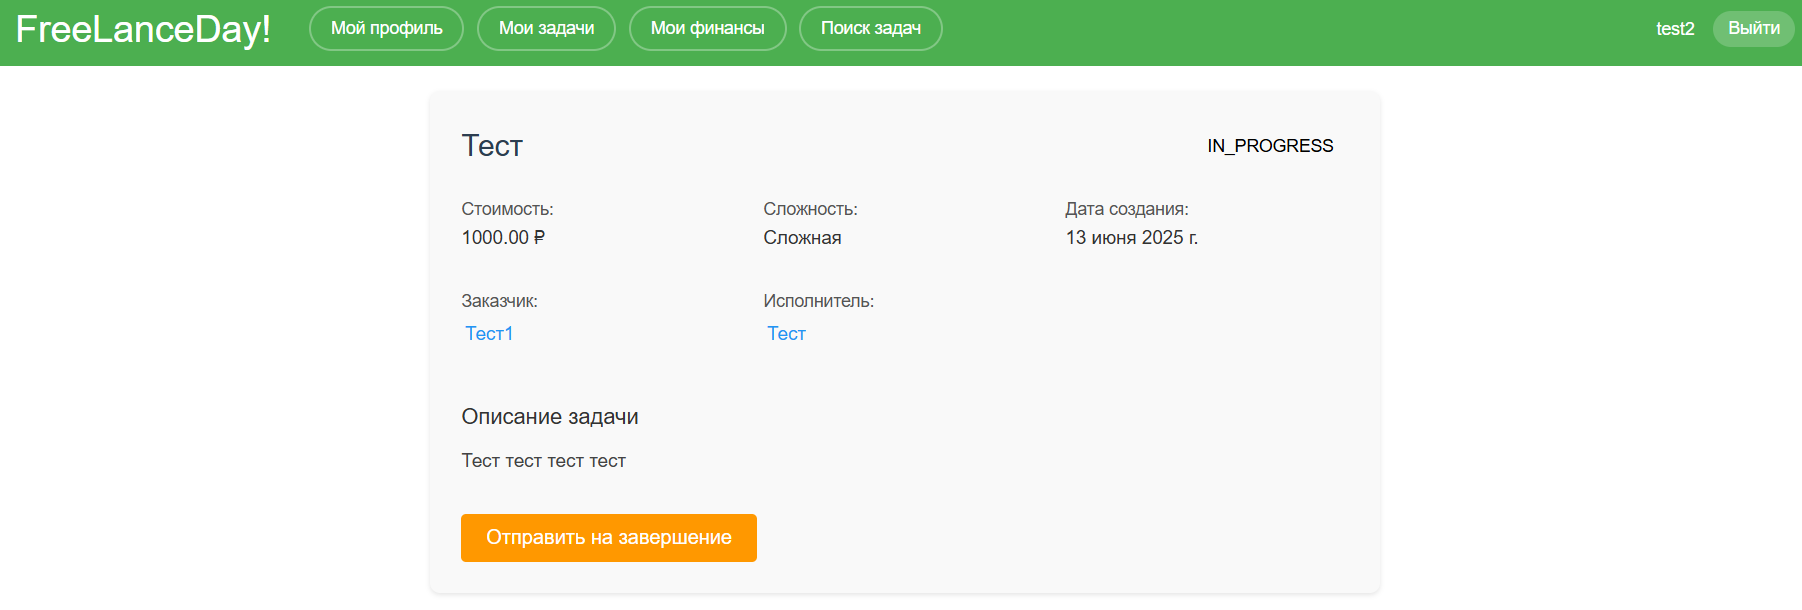
\includegraphics[width=1\linewidth]{t33.png}}
	\caption{Страница просмотра задачи исполнителем в статусе "<В работе">}
	\label{t33:image}
\end{figure}
\clearpage

\begin{figure}[ht]
	\center{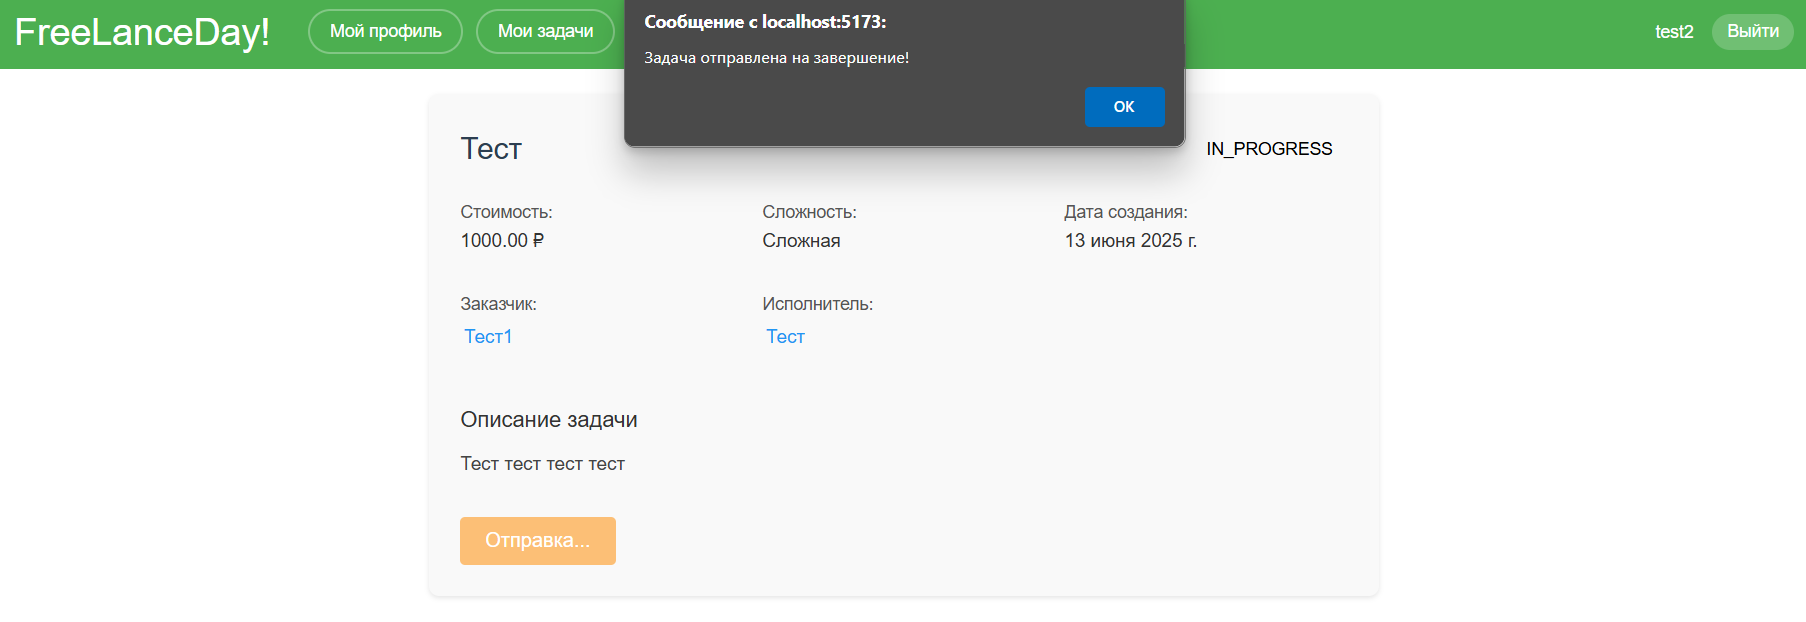
\includegraphics[width=1\linewidth]{t35.png}}
	\caption{Отправка задачи на завершение}
	\label{t35:image}
\end{figure}

\begin{figure}[ht]
	\center{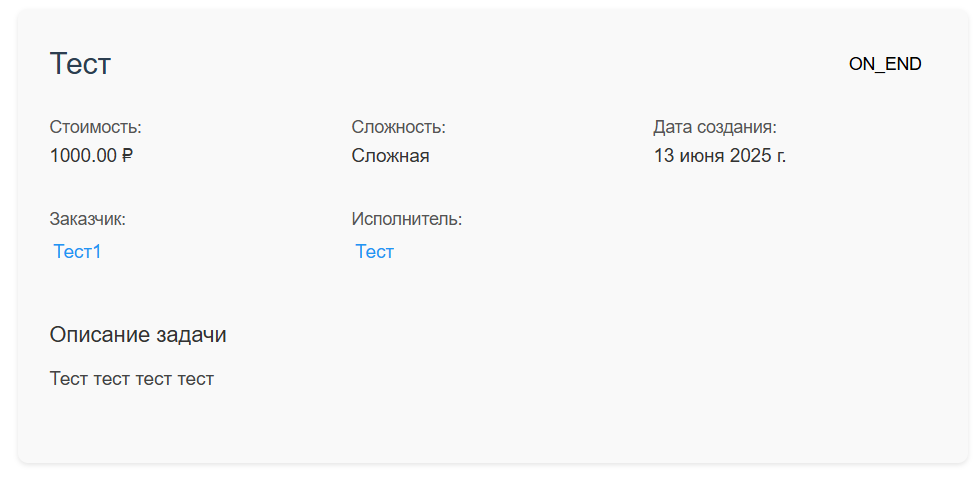
\includegraphics[width=1\linewidth]{t36.png}}
	\caption{Задача в статусе "<На завершении">}
	\label{t36:image}
\end{figure}

На рисунках \ref{t37:image}--\ref{t41:image} представлено завершение задачи заказчиком.
\clearpage

\begin{figure}[ht]
	\center{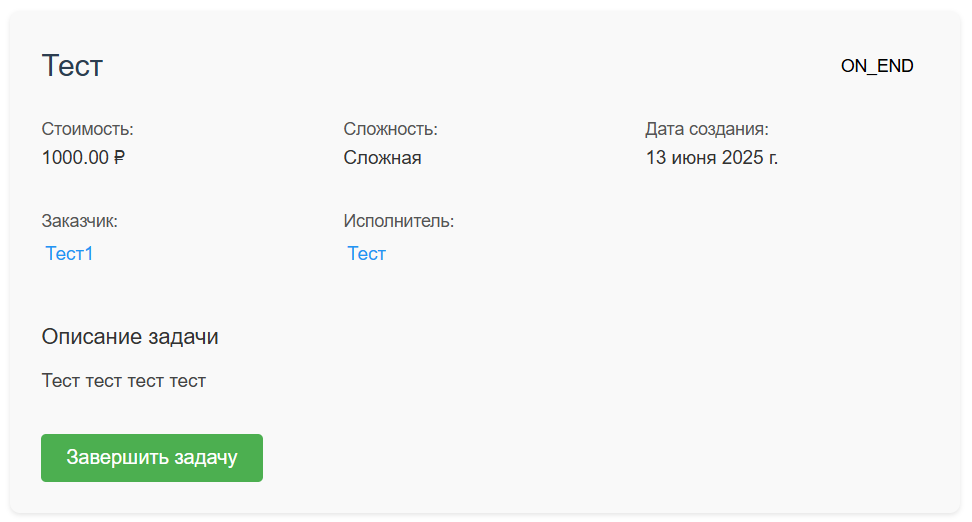
\includegraphics[width=1\linewidth]{t37.png}}
	\caption{Просмотр задачи в статусе "<На завершении"> заказчиком}
	\label{t37:image}
\end{figure}

\begin{figure}[ht]
	\center{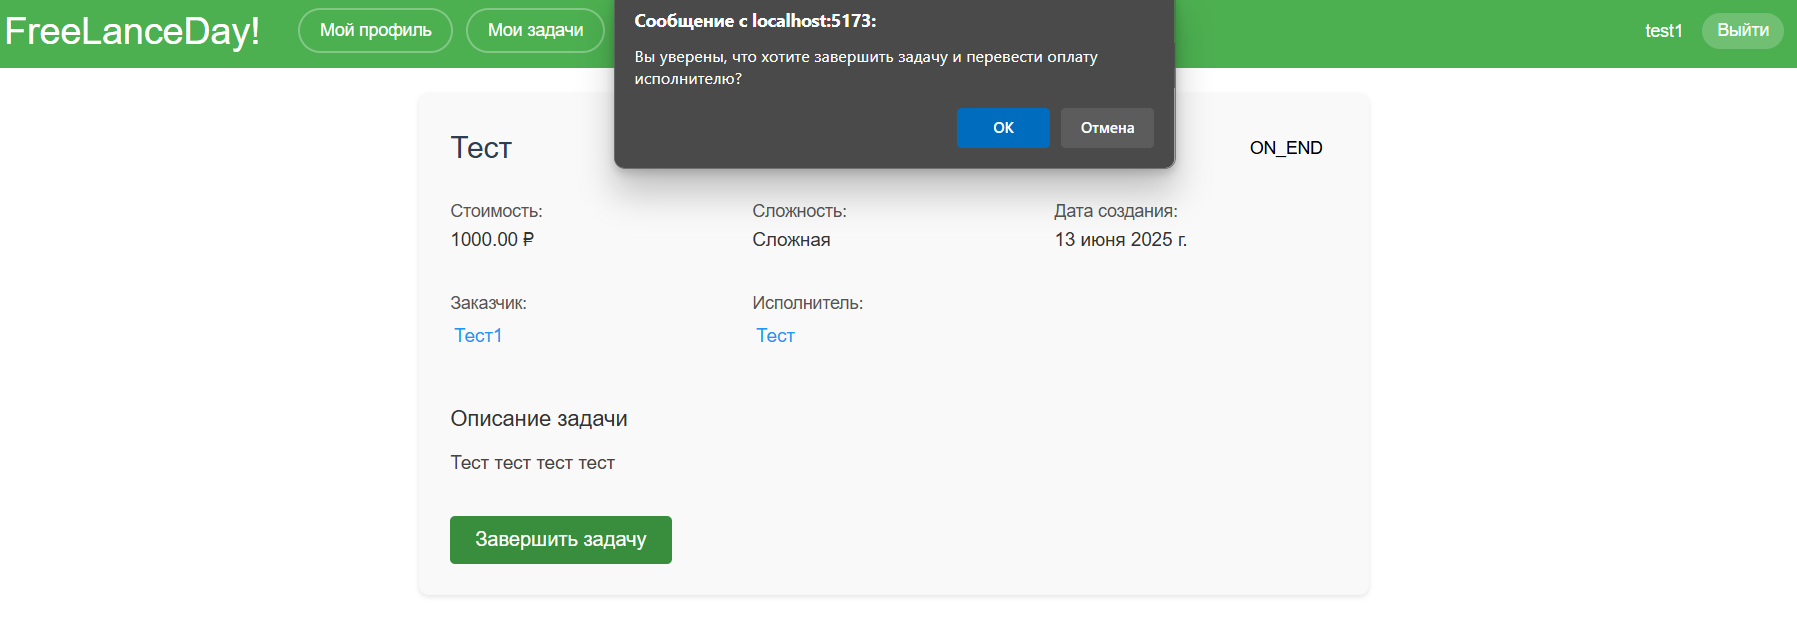
\includegraphics[width=1\linewidth]{t38.png}}
	\caption{Завершение задачи}
	\label{t38:image}
\end{figure}
\clearpage

\begin{figure}[ht]
	\center{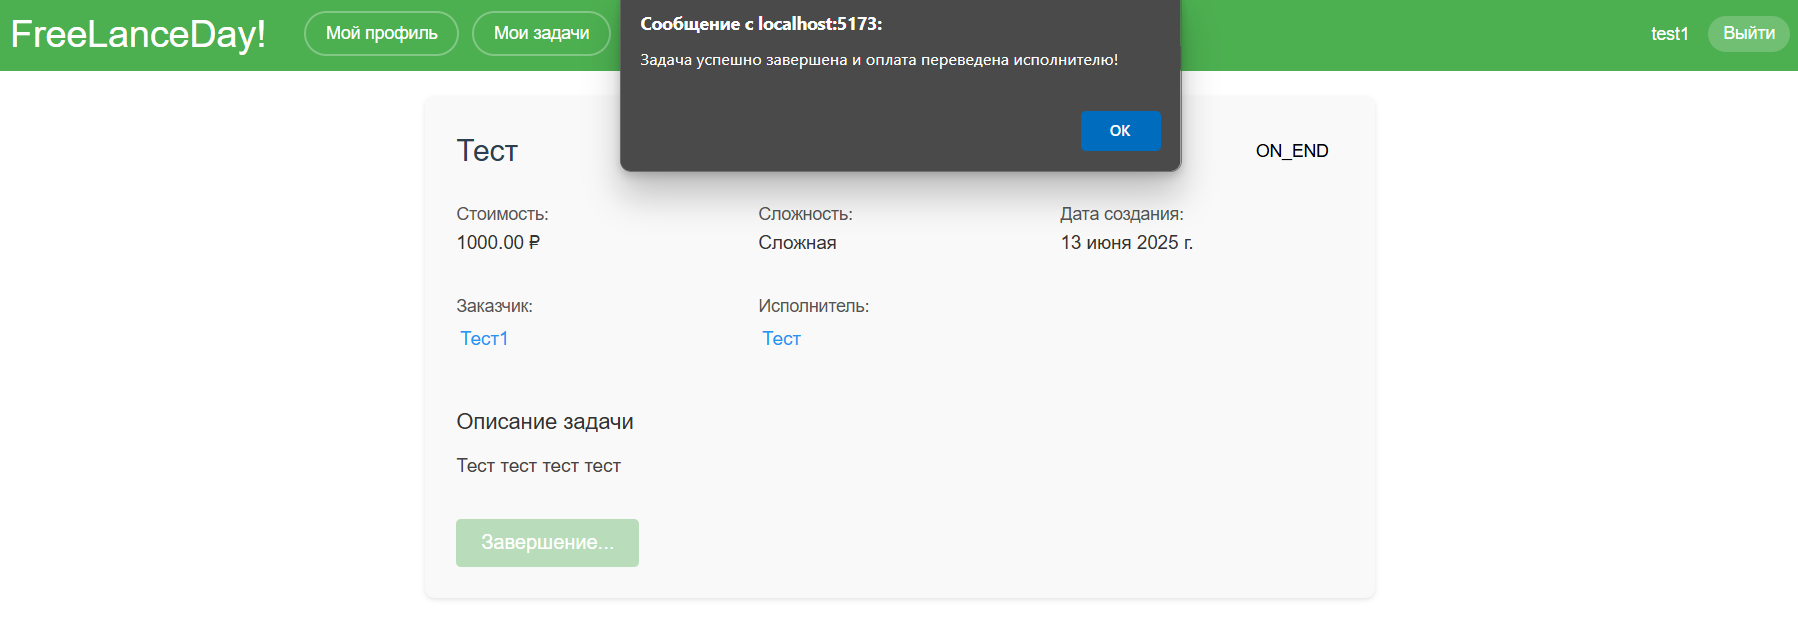
\includegraphics[width=1\linewidth]{t39.png}}
	\caption{Подтверждение завершения}
	\label{t39:image}
\end{figure}

\begin{figure}[ht]
	\center{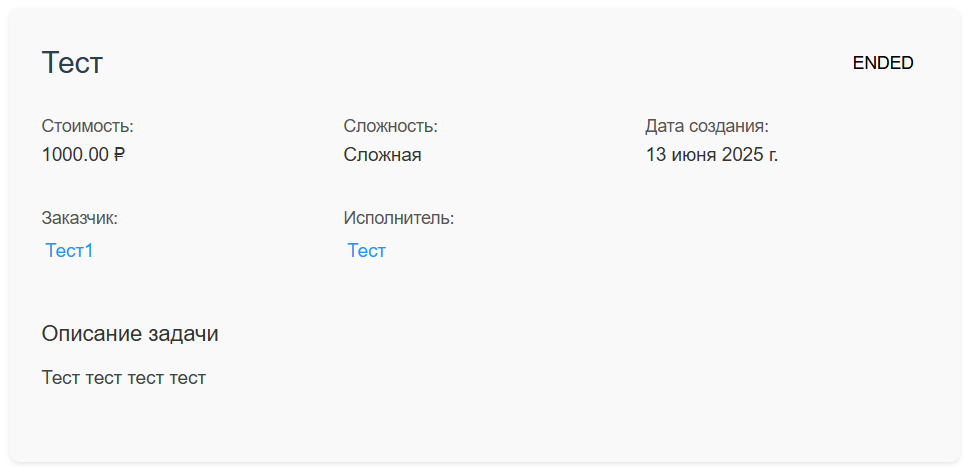
\includegraphics[width=1\linewidth]{t40.png}}
	\caption{Просмотр завершённой задачи}
	\label{t40:image}
\end{figure}

\begin{figure}[ht]
	\center{
\includegraphics[width=0.5\linewidth]{t41.png}}
	\caption{Завершённая задача не отображается в разделе "<Мои задачи">}
	\label{t41:image}
\end{figure}
\clearpage

На рисунках \ref{t42:image}--\ref{t47:image} представлен вывод средств с виртуального счёта исполнителя.

\begin{figure}[ht]
	\center{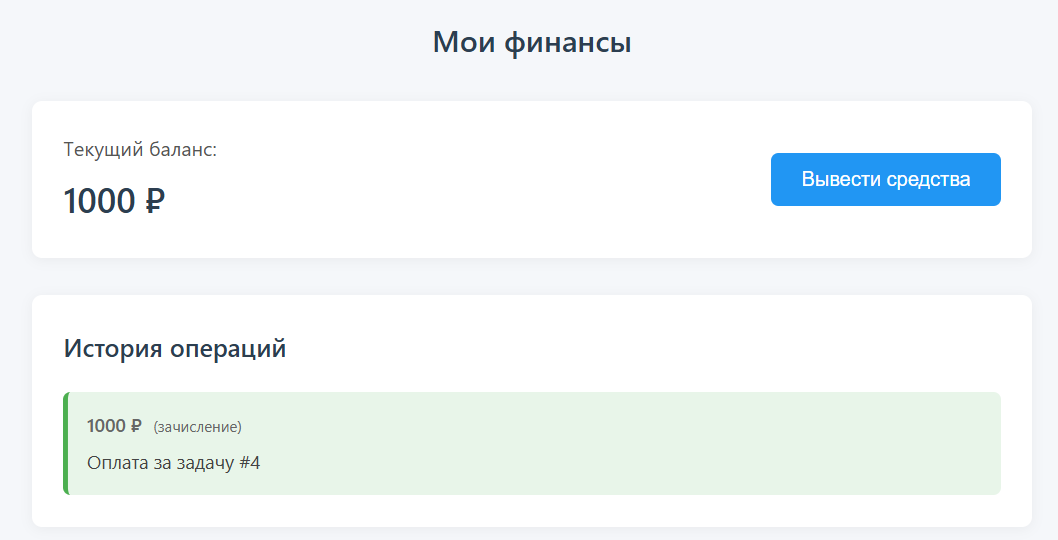
\includegraphics[width=1\linewidth]{t42.png}}
	\caption{Страница просмотра виртуального счёта исполнителя}
	\label{t42:image}
\end{figure}
\clearpage

\begin{figure}[ht]
	\center{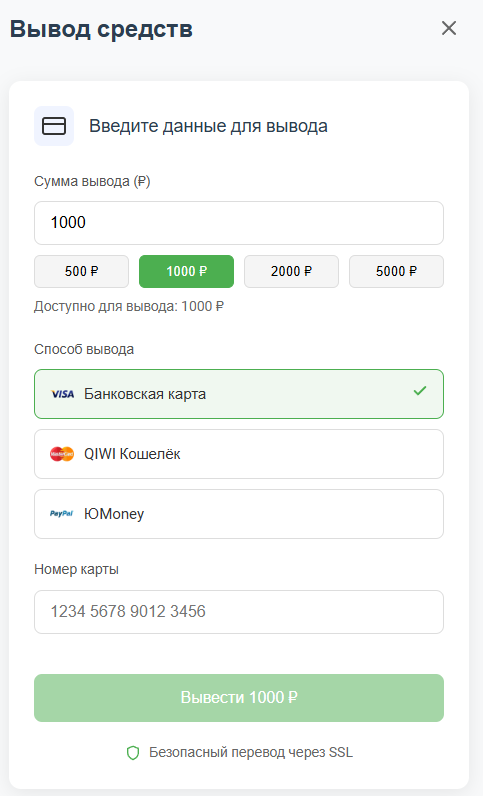
\includegraphics[width=0.7\linewidth]{t43.png}}
	\caption{Страница вывода средств с виртуального счёта}
	\label{t43:image}
\end{figure}
\clearpage

\begin{figure}[ht]
	\center{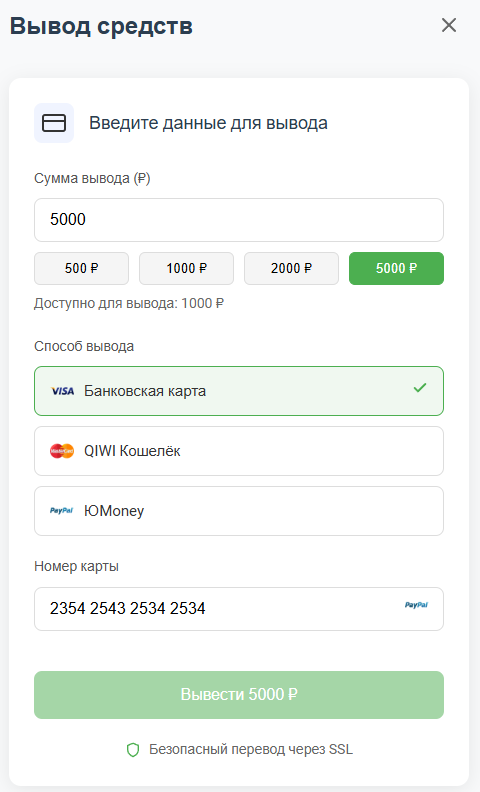
\includegraphics[width=0.7\linewidth]{t44.png}}
	\caption{Выбор суммы, превышающей сумму на балансе -- кнопка вывода средств не активна}
	\label{t44:image}
\end{figure}
\clearpage

\begin{figure}[ht]
	\center{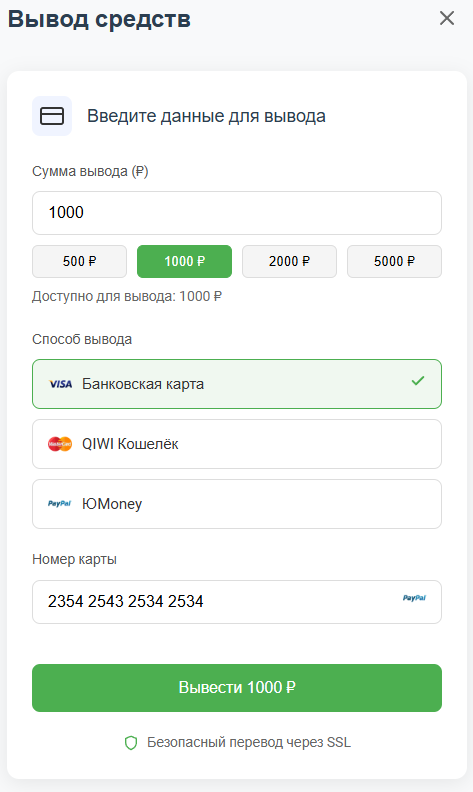
\includegraphics[width=0.7\linewidth]{t45.png}}
	\caption{Пример заполнения полей валидными значениями}
	\label{t45:image}
\end{figure}
\clearpage

\begin{figure}[ht]
	\center{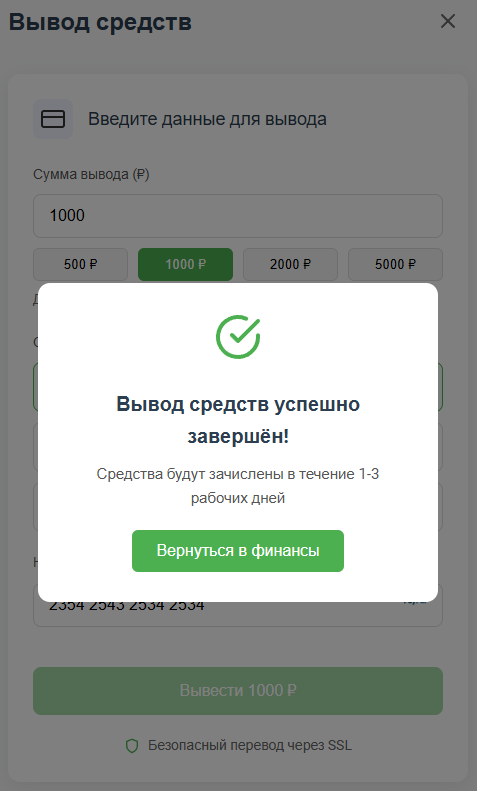
\includegraphics[width=0.7\linewidth]{t46.png}}
	\caption{Сообщение об успешном выводе средств}
	\label{t46:image}
\end{figure}
\clearpage

\begin{figure}[ht]
	\center{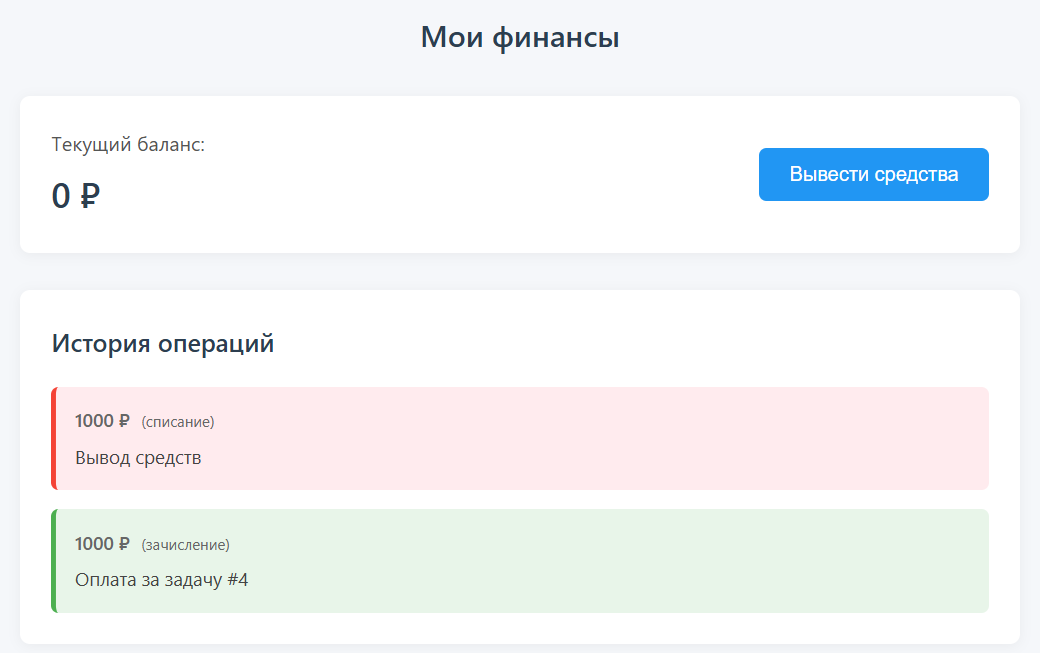
\includegraphics[width=0.7\linewidth]{t47.png}}
	\caption{Виртуальный счёт исполнителя после вывода средств}
	\label{t47:image}
\end{figure}

На рисунках \ref{t48:image} и \ref{t49:image} представлен пример выхода из аккаунта пользователя.

\begin{figure}[ht]
	\center{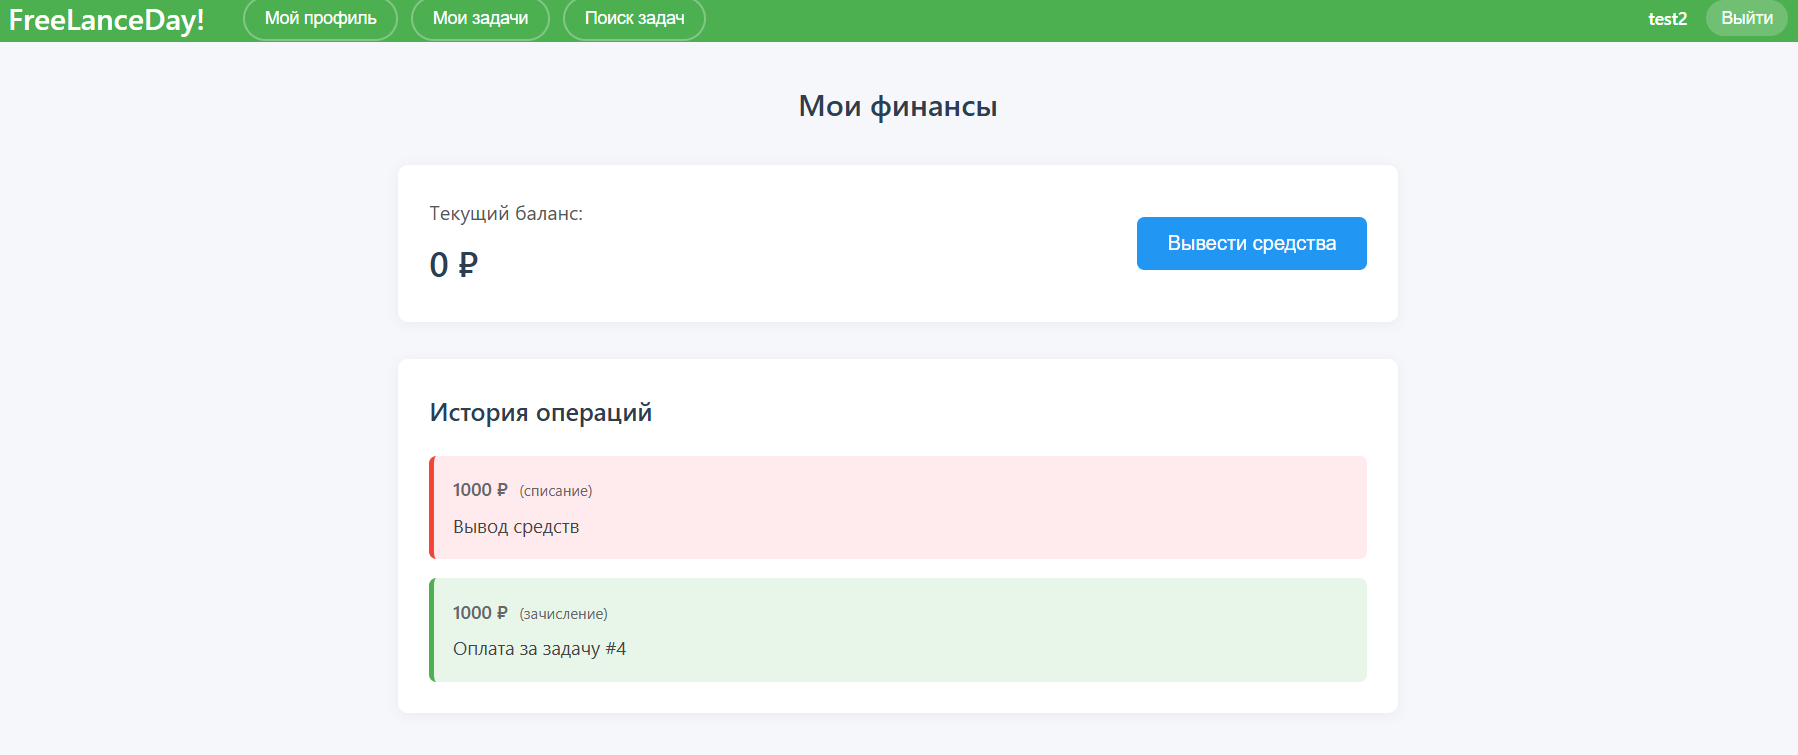
\includegraphics[width=1\linewidth]{t48.png}}
	\caption{Страница просмотра виртуального счёта, в правом верхнем углу отображается кнопка "<Выйти">}
	\label{t48:image}
\end{figure}

\begin{figure}[ht]
	\center{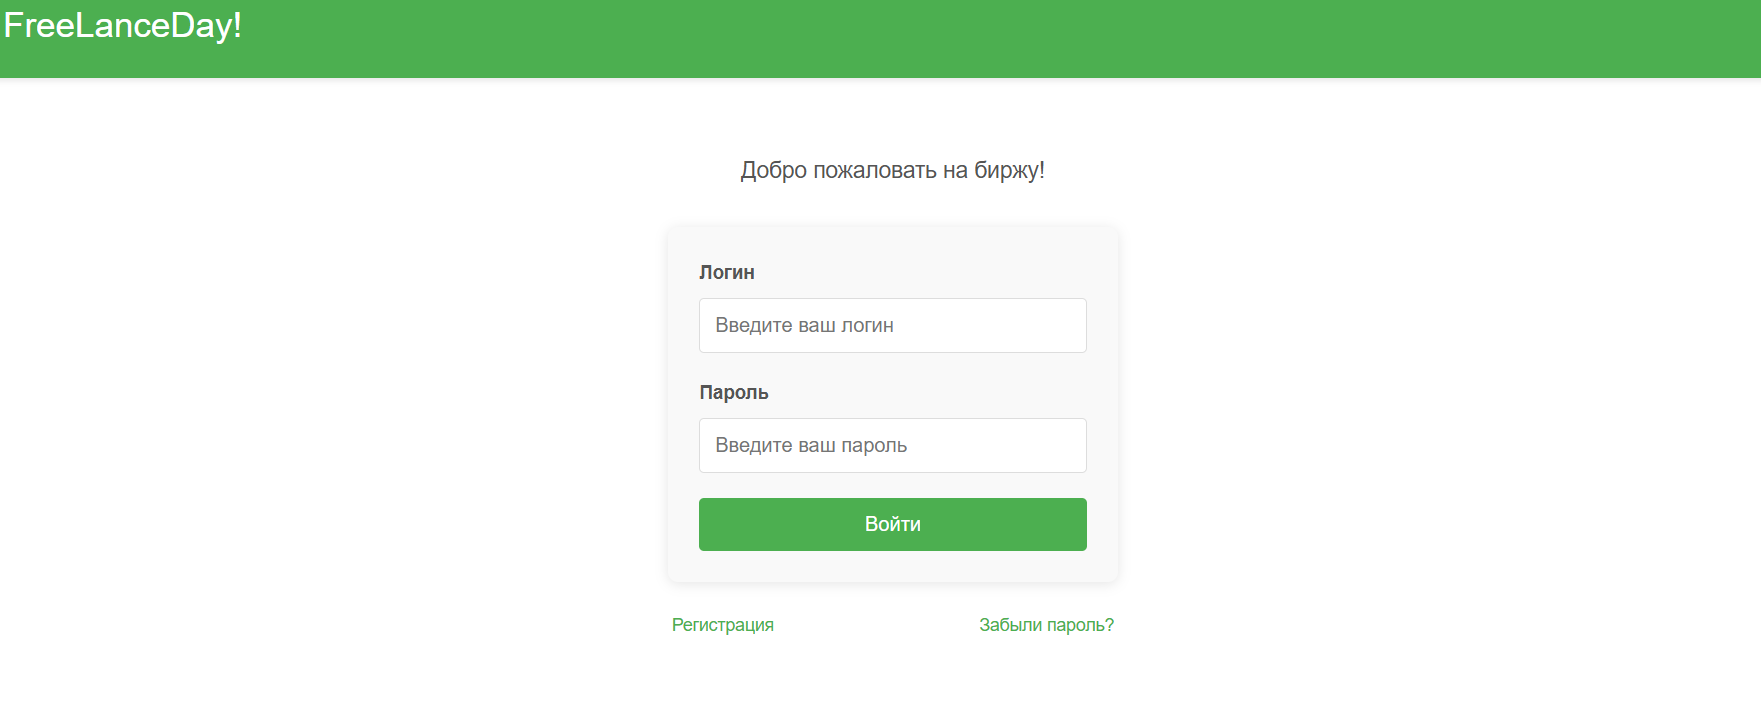
\includegraphics[width=1\linewidth]{t49.png}}
	\caption{После нажатия кнопки "<Выйти"> отображается страница авторизации}
	\label{t49:image}
\end{figure}

\clearpage